\documentclass[a4paper]{article}

\usepackage[T1]{fontenc}
\usepackage[utf8]{inputenc}
\usepackage[italian]{babel}
\usepackage{amssymb}
\usepackage{hyperref}
\usepackage{mathtools}
\usepackage{amsthm}
\usepackage[ruled,vlined,noend]{algorithm2e}

% ===== Graph =====
\usepackage{tikz}
% ===== multicol =====
\usepackage{blindtext}
\usepackage{multicol}
% ===============

\mathtoolsset{showonlyrefs}  
\hypersetup{
    colorlinks=true,
    linkcolor=black,
    filecolor=black,      
    urlcolor=black,
}

\newcommand{\pluseq}{\mathrel{{+}{=}}}

\newtheorem{theorem}{Teorema}
\newtheorem{corollary}{Corollario}
\newtheorem{lemma}{Lemma}
\newtheorem{remark}{Osservazione}
\newtheorem{definition}{Definizione}

\setcounter{secnumdepth}{3}
\setcounter{tocdepth}{3}

\title{Parallel and Distributed Algorithms.tex}
\author{Federico Bruzzone}
\makeindex
\begin{document}
\maketitle
\newpage
% \setlength{\parskip}{0.15em}
\tableofcontents
\setlength{\parindent}{0pt}
\setlength{\parskip}{0.8em}
\newpage


\section{Overview}

The assignment is focused on implementing a simple Architecture using Python Abstract Classes to build a structure that is lead to retrieve data from generics externals data source for importing them into an internal DB that will be used from the analyst’s team for analysis purposes.

\section{Project Requirements}

The project requirements are reduced to the ideation and abstract implementation of a software architecture which satisfies to follow the \textit{Software Architecture Pillars} seen during the class lessons.

In specific those pillars are:

\begin{enumerate}
	\item Being the framework for satisfying requirements
	\item Being the technical basis for design
	\item Being the managerial basis for cost estimation and process management
	\item Enabling component reuse
	\item Allowing a tidy scalability 
	\item Avoiding handover and people lock in
\end{enumerate}

\section{Software Architecture Pillars}

\subsection{Being the framework for satisfying requirements}

\begin{center}
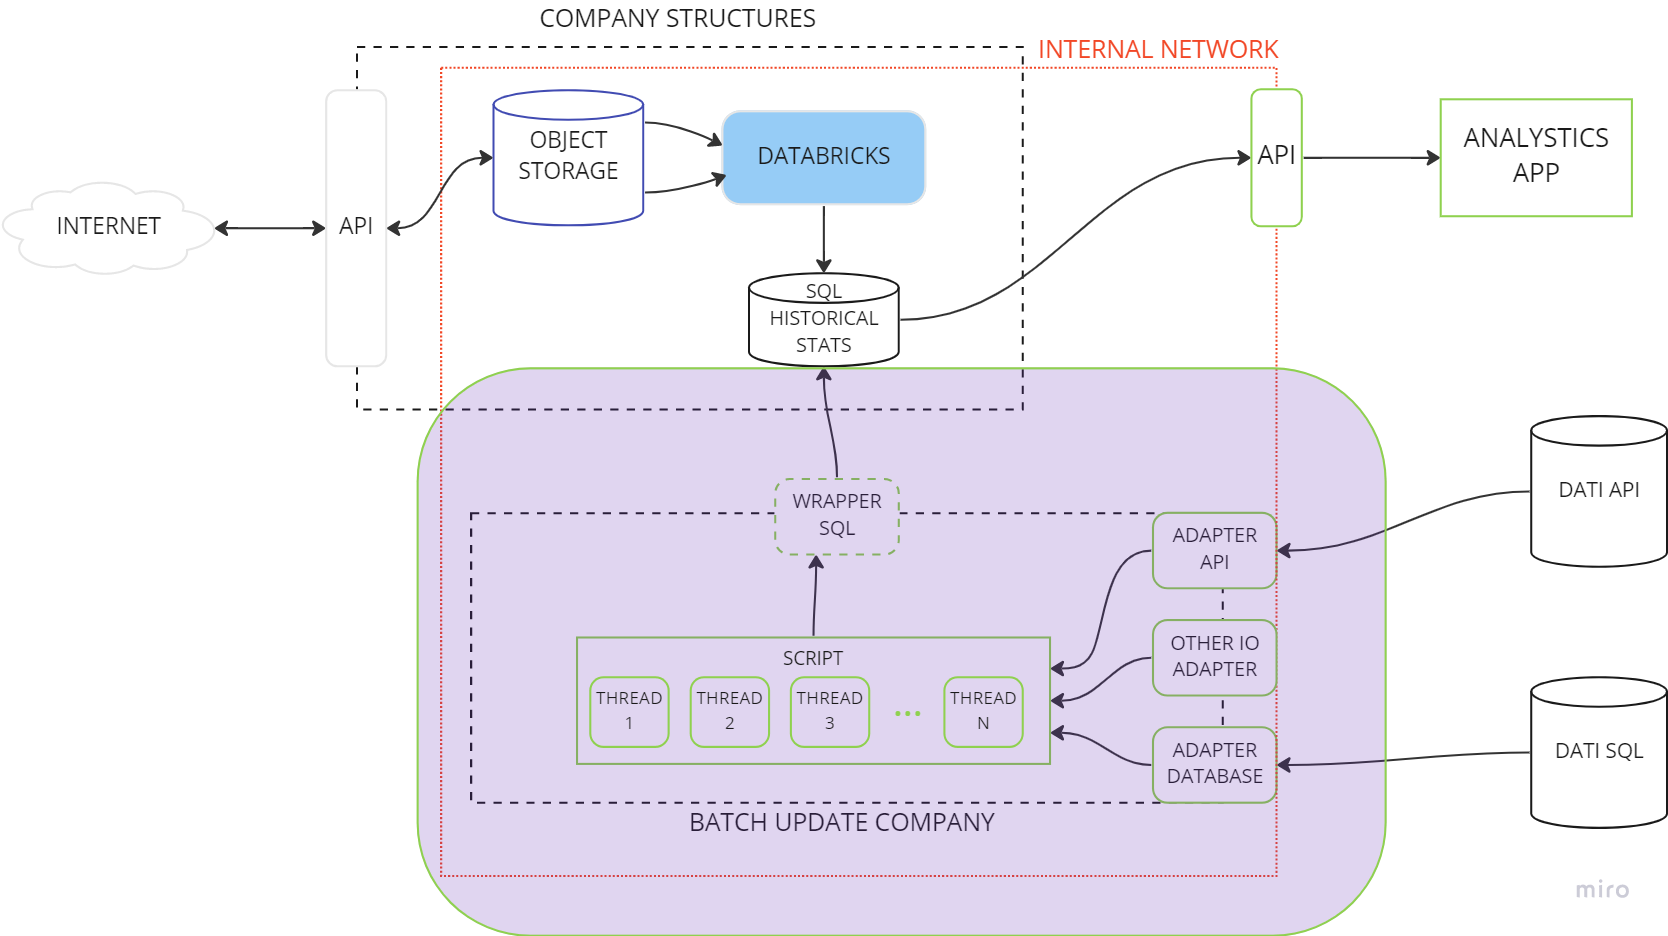
\includegraphics[scale=0.4]{scheme-diagram}
\end{center}

\subsubsection{Functional Requirements}

The software will need the ability to read data from generic external sources (like Databases, public API, Data Stream, …) and to prepare and process them before their insertion inside the local Company Historical DB.

This software, that furthermore we will call ‘Batch Extractor’, will need to be able to adapt itself for retrieving data from any data source that the company will identify as important to be importable inside the system for allowing analysts to be free of finding whatever data source should fit better for their needs.

The batch system will also need to be adaptable for changes on the internal structure of the Company, in particular the DB, for letting free the company to make the best business and behavioral choices in any moment free of the current implementations of the system.

Important will also be that the structure should be scalable on multiple and concurrent input data source, for allowing the system to inject data at different speeds based on the need of the analyst and the environment.

\subsubsection{Technical Requirements}

Due to accomplish the necessity of the structure of being adaptable to any external source, is important that the software will presents a layer of external adapters that will be used to connect to the external sources for retrieving properly data based on the external infrastructures and needs. 

Important will also be the possibility for the system to be able to add new adapters to interact with new outside data sources. Those will simply need to pass the data to the script unknowingly of the internal DB implementation and this will then take care of them for the inserting inside the Historical DB.

Important will also be the presence of wrappers for the connection with the internal Historical DB. 
This feature will provide another abstraction layer that will be important to allow the company to apport in any moment whatever changes on the internal technologies used for storing data.

\subsubsection{Security Requirements}

The system will need to be placed inside the company network due to avoid the necessity of opening external ports directly to the Historical DB, for reduce the possibility of penetration of malicious actors inside the system.

Important will also be the process of input sanitization after receiving data from the external source and before inserting them inside the queries, due to avoid the exposure of the system to attack like SQL injection or similar.

\subsection{Being the framework for satisfying requirements}

The development of the architecture, later illustrated, has been done keeping in mind that we will have a single immutable database (historical database) on which we will write and possible multiple databases or data sources from which we will read.

To interface on these databases (or data sources) we thought to use multiple adapters to transform the inbound data in a writable format for the Historical DB.

\begin{center}
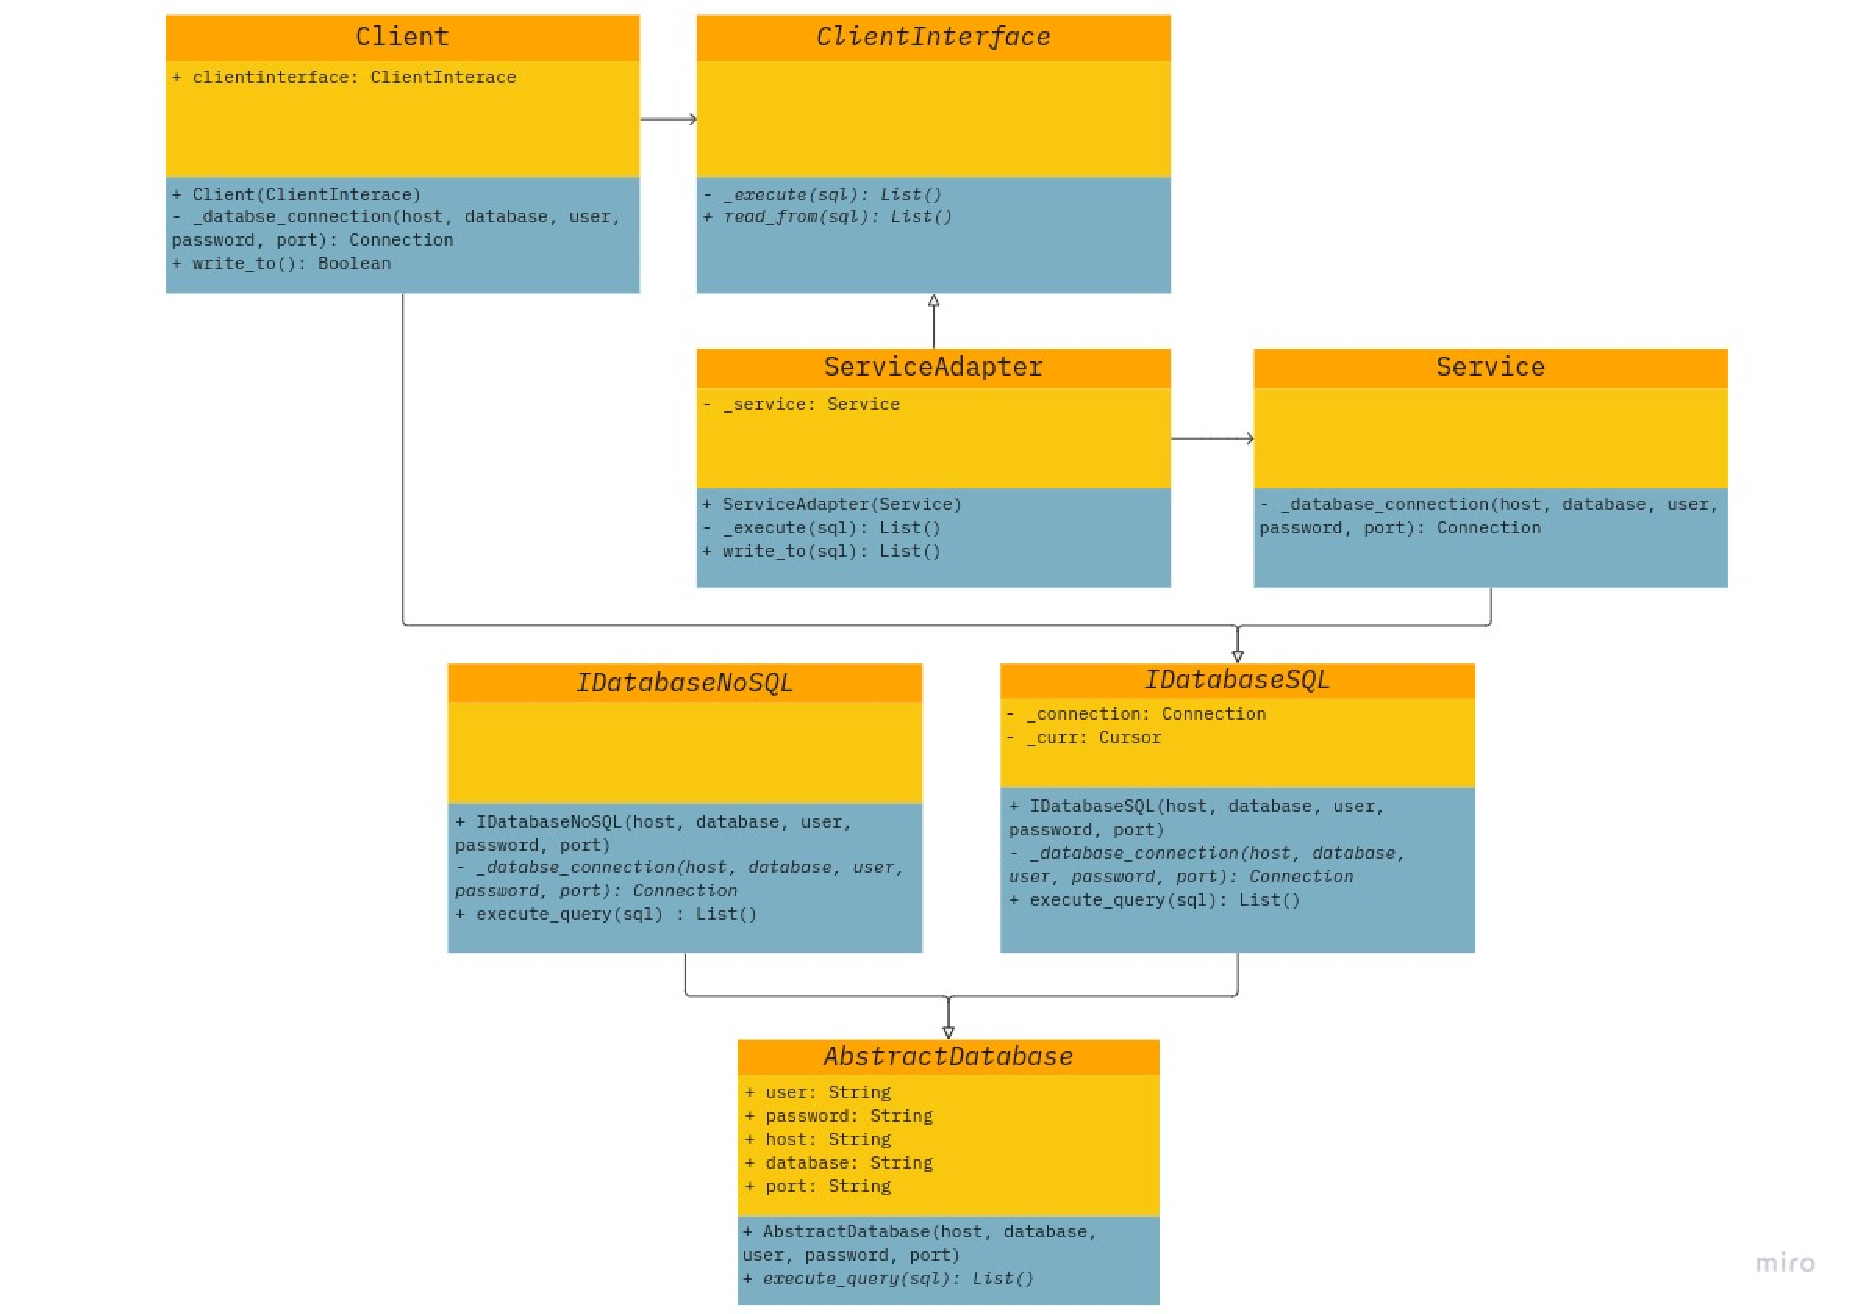
\includegraphics[scale=0.45]{uml-diagram}
\end{center}

\textbf{Please note: The gray part is not implemented. We will talk about it in the reusability chapter.}

We have thought to use Adapter (Wrapper) pattern, because this will allow us to keep the same historical database and make it be able to communicate with the different types of external data source.

This implementation uses the object composition principle: the adapter implements the interface of one object and wraps the other one.

\begin{enumerate}
	\item \textit{AbstractDatabase} is an abstract class that contains the information for connecting with any database.
     
     In the inherited class, you will have to implement execute\_query(...) method.

	\item \textit{IDatabaseSQL} is an abstract class that define behavior of the SQL database.
     
     Since IDatabaseSQL inherits from AbstractDatabase it must implements execute\_query(...) method.
     
     In the inherit class, you will have to implement \_database\_connection(...) method.

     Assuming that in python any database sql library implement .connector.connect(...) and .cursor() methods: 
\begin{enumerate}
	\item we use \_connection field to store the connection to the specific database;
	\item we use \_cursor field to store the cursor to the specific database.
\end{enumerate}

Note that \_cursor contanis the .execute(...) method that is used to execute the query.

	\item \textit{ExternalDatabase} is a concrete class that allow us to establish a connection.
	
     Since ExternalDatabase inherits from IDatabaseSQL it must implements \_database\_connection(...).

	\item \textit{ExternalDatabaseAdapter} is a concrete class that allow data from ExternalDatadase to be readable and writable for HistoricalDatabase. 
	
     Since ExternalDatabaseAdapter inherits from IHistoricalDatabse it must implements \_read\_from(...) and \_execute(...) methods.
     
     Since ExternalDatabaseAdapter has an ExternalDatabase object instance inside, it will have the ability to execute query from it and therefore having the ability to read data from it.

	\item \textit{IHistoricalDatabse} is an interface that contains the delcarations of methods that must be implemented by each adapters.
	
     We expect the read\_from(...) mothod to return a fitted content for the HistoricalDatabase. 

	\item \textit{HistoricalDatabse} is a concrete class that contains methods to execute query into the historical database.
	
     Since HistoricalDatabse inherits from IDatabaseSQL it must implements \_database\_connection(...).
    
     Since HistoricalDatabse has a IHistoricalDatabase object it can get data from it.
     
     To remember the last item we have read, we store its identifier (ordered) into a sync.json file, and when we will have to execute the next query, we'll read from sync.json the identifier.
        
     The .write\_to(...) mothod use the .read\_from(...) method of the adapter to get a list of tuple and then insert them into the historical database. 
     
     After this, it will commit the changes.
\end{enumerate}

\subsection{Being the managerial basis for cost estimation and process management}

\begin{lstlisting}[language=Python, numbers=none]
Infrastructure Cost: Physical Server owning:    4 x 9000$ = 36000$
                     Estimated power:           4 x 250$ = 1000$/month
                     Estimated internet access: 2250$/month
     Developer Cost: 3 Agents:                  30000$
                     Software developing:       35000$
                     Network adapt:             20000$
 Algorithmical Cost: Business logics:           10000$
   Maintenance Cost:                            20000$/Year


        TOTAL COSTS: One Shot:                  131000$
                     Running:                   57K000/Year 
\end{lstlisting}

\textbf{Infrastructure Specs}

Physical Server: 4 * ProLiant DL385 Gen10 Plus : 9,000.00 

Power costs:     4* 1600W (Server alimentation) = 6400W * 13c\$/KwH : 1000\$

Internet costs:  Dedicated Internet Access, 40Gbps IP Transit: 2250\$/month

Developer cost:  Based on 6 months working\\

\subsection{Enabling component reuse}

\begin{lstlisting}[language=Python]
class IHistoricalDatabse(ABC):
    @abstractmethod
    def _execute(self, sql): pass

    @abstractmethod
    def read_from(self, sql): pass

class ExternalDatabaseAdapter(IHistoricalDatabse):
    external_databse: ExternalDatabase = ''

    def __init__(self, external_databse: ExternalDatabase):
        self.external_databse = external_databse
        print('ExternalDatabaseAdapter has been created')

    def _execute(self, sql):
        query_res = self.external_databse.execute_query(sql)
        return query_res
    
    def read_from(self, sql):
        query_res = self._execute(sql) 
        return query_res   
\end{lstlisting}

Talking about reusability, as you can see in the uml diagram in chapter 1.2, the not implemented gray parts are just examples of external sources that could be implemented if we will need to read from other services. 

Doing so we we'll not have to change each time the way we are going to write into the internal DB, because the adapter will achieve the goal to manage the importing of data inside the script. From here then the data will be passed by the wrapper to the internal DB.

Obviously, it you want to create a new adapter, you will have to code a class which will inherit from IHistoricalDatabase. This allow the historical database, which contains an IHistorical database object, to not change the internal code.

\subsection{Allowing a tidy scalability}

The system has been ideated and structured to be scalable on the quantity of data received in input from the external sources.
This choice born from the unknown of the availability of data during time on the remote source.

Allowing this scalability help the system to be ready for situations where the data are given “real time” and are not retrievable in a second moment. For not losing data will be important for the system to be able to adapt his capability of reading data without losing on performance or reliability.

At this purpose the script will have more internal threads that will be capable of increasing in number when there will be high inbound traffic and then reduce themselves when not anymore necessary.

\subsection{Avoiding handover and people lock-in}

The problem of vendor lock-in is commonly forcing the company to be stuckked to use some internal technologies that cannot be changed because the cost of the replacement would be higher than the benefits. This problem can also raise on company’s employees when the develop of code has not been well documented and the company find herself to be in the position to cannot replace an employee due to his only known about the project code.

To avoid those problem the solution proposal has been to implement an internal wrapper between the script and the internal DB to allow in a second moment to be able to change internal technologies configurations and from the employees prospective we provide a fully code documentation to let any new future worker on the project be able to understand every snip of code what is doing and how to manage them in case of bug or unexpected behavior.

\section{Testing}

We have tested the code by creating table \textbf{user1} and \textbf{user2} with \textit{id} (Primary Key, Auto Increment), \textit{name} and \textit{surname} respectively and then we have tried to read from \textbf{user1} and write to \textbf{user2}.

We have used sync.json file to store the last tuple that we have read from the \textbf{user1}.

Reading this file we were able to resume reading \textbf{user1} from the last writing in table \textbf{user2}, whitout reading the whole database every time.

For simplicity, we have been using the id of the \textbf{user1} table to keep track of the last tuple stored in the sync.json file, and we have read and wrote in the same database instance.

Our tests were performed succesfully.


\textbf{First execution}
\begin{lstlisting}
Connection successfull to the: 
          127.0.0.1 test_database root welcome123 
ExternalDatabaseAdapter has been created
Connection successfull to the: 
          127.0.0.1 test_database root welcome123 

Query has been executed: 
          SELECT name, surname FROM user where id > 0
          ('federico', 'bruzzone')
          ('andrea', 'longoni')
          ('massimiliano', 'visconti')

Query has been executed: INSERT INTO user2 (name, surname) 
                         VALUES ('federico', 'bruzzone');

Query has been executed: INSERT INTO user2 (name, surname) 
                         VALUES ('andrea', 'longoni');

Query has been executed: INSERT INTO user2 (name, surname) 
                         VALUES ('massimiliano', 'visconti');
\end{lstlisting}


\textbf{Second execution}

The second execution did not write data since in the user1 table there are only three tuples and in our sync.json the counter was setted to three after the first execution.

\begin{lstlisting}
Connection successfull to the: 
          127.0.0.1 test_database root welcome123 
ExternalDatabaseAdapter has been created
Connection successfull to the: 
          127.0.0.1 test_database root welcome123 

Query has been executed: 
          SELECT name, surname FROM user where id > 3
\end{lstlisting}

%\section{Algoritmi di approssimazione}
In questa parte si introdurranno gli algoritmi di approssimazione, 
dopo aver accennato ad alcuni concetti preliminari legati alla complessità.
Si definiranno in particolare classi di problemi e alcune 
tecniche note nella risoluzione di problemi di ottimizzazione.

\subsection{Notazioni}

\paragraph{Insiemi numerici come interi}
Si indicheranno alcuni insiemi numerici con un singolo intero, 
es $$k = \{0, 1, \dots, k-1\}$$

\paragraph{Insieme delle funzioni} L'insieme delle funzioni che hanno come dominio $A$ e codominio $B$ si indica come segue: 
$$B^A = \{ f | f : A \rightarrow B\}$$

\paragraph{Insieme delle parti} L'insieme dei sottoinsiemi di $A$ si indica con $2^A = P(A)$.

\paragraph{Alfabeto} Fissato un alfabeto $\Sigma$, indichiamo con $\Sigma^*$ l'insieme delle stringhe ottenute da 
$\Sigma$.

\paragraph{Esempio}
La notazione $2^{2^*}$ indica l'insieme dei linguaggi binari.

\subsection{Classi di complessità}
Partiamo dalla definizione di algoritmo, per poi arrivare a definire la 
complessità algoritmica e strutturale.
\paragraph{Algoritmo}
Un algoritmo per un problema $\Pi$ è una macchina di Turing, che verrà indicata con $A$, che opera come segue:
$$x \in I_{\Pi} \longrightarrow A \longrightarrow y \in O_{\Pi}\;\;t.c.\;\;y \in Sol_{\Pi}(x)$$
$$Sol_{\Pi}: I_\Pi \longrightarrow (2^{O_\Pi} \setminus \{\emptyset\})$$
La funzione associa ad un input l'insieme dei suoi output corretti.

\begin{remark}
    Gli input di un problema devono essere codificati in qualche modo. 
    Ad esempio, considerando una macchina di Turing, gli input sono 
    pensati come stringhe binarie. 
    Esistono molti modi di codificare per esempio due interi, si potrebbe pensare di utilizzare la coppia di Cantor, oppure di raddoppiare i bit.
    La complessità di un algoritmo non varia se le codifiche sono 
    polinomialmente contenute le une nelle altre. Ovvero, una codifica esponenziale cambierebbe la complessità rispetto a una codifica polinomiale, 
    ma nel nostro caso non succederà.
\end{remark}

\subsubsection{Complessità algoritmica}
La complessità algoritmica è lo studio del dispendio di risorse di 
un algoritmo. Sostanzialmente ci si sta chiedendo come un algoritmo risolve un certo problema.

Una delle risorse considerabili è il tempo: $$T_A : I_\Pi \rightarrow \mathbb{N}$$
Alternativamente possiamo considerare questa funzione, che ragione per taglia piuttosto 
che per singolo input: 
$$t_A : \mathbb{N} \rightarrow \mathbb{N}$$ dove il dominio è 
la lunghezza di input, in quel caso si avrà che 
$$t_A(n) : \max\{ T_A(x),\; x \in I_{\Pi},\; |x| = n\}$$

Si possono considerare limiti alla complessità algoritmica, un upper bound si ottiene 
esibendo una soluzione con quella complessità, per esempio, trovo una soluzione quadratica 
al problema dell'ordinamento. Posso anche trovare un lower bound, per esempio, 
dimostro che ordinare $n$ valori richiede almeno $O(n \log n)$ operazioni.

\subsubsection{Complessità strutturale}
Si definiscono ora due classi di problemi, \emph{P} e \emph{NP}, per 
poi introdurre i concetti di \emph{riducibilità polinomiale} e di \emph{NP-completezza}.

\paragraph{Classe P}
La classe \emph{P} corrisponde ai problemi decisionali 
per cui esiste un algoritmo che opera
in tempo polinomiale, ovvero: 
$$P = \{\Pi\;|\;\Pi\;decisionale, \; \exists\;A\;per\;\Pi,\;t.c.\;t_a(n)\;=\;O(Polinomio)\}$$

\paragraph{Classe NP}
La classe \emph{NP} corrisponde ai problemi decisionali 
per cui esiste un algoritmo che opera
in tempo polinomiale su una macchina non deterministica, ovvero: 
\begin{equation}
    \begin{aligned}
        \mathit{NP} = \{\Pi\;|\;\Pi\;decisionale, \; \exists\;A\;per\;\Pi,\; t.c.\;t_a(n)\;=\;O(Polinomio)\;
        \\su\;una\;macchina\;non\;deterministica\}
    \end{aligned}
\end{equation}

\begin{remark}
    Un problema è decisionale se dato un input da un output binario.
\end{remark}

\paragraph{Riducibilità polinomiale}
Un problema $\Pi_1$ si dice riducibile polinomialmente ad un problema $\Pi_2$ se esiste 
un mapping tra input del primo e del secondo problema che rispetta le seguenti proprietà:
$$\Pi_1 \leqslant _p \Pi_2 \;sse\; \exists f : 2^* \rightarrow 2^*\; t.c$$
\begin{enumerate}
    \item $f$ è calcolabile in tempo polinomiale
    \item $\forall x \in I_{\Pi1},\;f(x) \in I_{\Pi2},\; Sol_{\Pi1}(x) = Sol_{\Pi2}(f(x))$ 
\end{enumerate}

\paragraph{NP completezza}
Un problema $\Pi$ è NP completo sse $\forall\;\Pi^\prime \in NP,\; \Pi^\prime \leqslant _p \Pi, \; \Pi \in NP$.
Ovvero se ogni problema in NP è riducibile polinomialmente al problema che si sta 
considerando.

\begin{theorem}
    SAT è NP completo.
\end{theorem}
\begin{corollary}
    Se $\Pi_1 \leqslant _p \Pi_2$ e $\Pi_1$ è NP completo, allora $\Pi_2$ è NP completo.
\end{corollary}
\begin{proof}
    $\Pi^\prime \in NP, \Pi^\prime \leqslant _p \Pi_1 \leqslant _p \Pi_2$, quindi $\Pi_2$ è NP completo.
\end{proof}
\begin{remark}
    Se trovassi un problema $\Pi$ NP completo t.c, $\Pi^\prime \leqslant _p \Pi$, 
    allora \emph{P=NP}.
\end{remark}

\subsection{Problemi di ottimizzazione}
Nella definizione di un problema di ottimizzazione bisogna tenere conto dei 
seguenti parametri:
\begin{enumerate}
    \item Insieme di input $I_\Pi \subseteq 2^*$;
    \item Insieme di output $O_\Pi \subseteq 2^*$;
    \item $F_\Pi : I_\Pi \rightarrow 2^{O_\Pi} \setminus \{\emptyset\}$, $F_\Pi(x)$ indica 
    le soluzioni accettabili per l'input $x$;
    \item $C_\Pi : I_\Pi \times O_\Pi \rightarrow \mathbb{Q}^{>0}$, funzione obiettivo, 
    con $C_\Pi(x,y)$ si indica il valore della funzione obiettivo per l'input \emph{x}, con soluzione $y \in O_\Pi$;
    \item $t_\Pi \in \{min, \;max\}$, ovvero il criterio del problema.
\end{enumerate}
L'insieme delle soluzioni per $x$ si può definire come:
$$Sol(x) = \{y^* \in O_\Pi | y^* \in F_\Pi, \forall y^\prime \in F_\Pi, c(x, y^*) \leqslant (\geq ) c(x, y^\prime)\}$$
Ovvero l'insieme delle $y$ possibili per quella fissata $x$, tale che minimizzano o massimizzano la funzione $C_\Pi$.

\paragraph{Problema di decisione associato}
Dato un problema di ottimizzazione $\Pi$ esiste un problema di decisione associato $\hat{\Pi}$.
\\L'idea è quella di considerare un input del problema originale e un costo alla soluzione, e rispondere
in base all'esistenza di una soluzione con quel costo.\\
In particolare: $$I_{\hat{\Pi}} = I_\Pi \times \mathbb{Q}^{>0}$$ 
$$(x, \theta) = C_\Pi(x, y^*(x)) \leqslant (\geq ) \theta$$

Ovvero, rispondo sì se e solo se il costo della soluzione ottima è minore, 
o maggiore, di $\theta$.
Pensando al problema MaxSat, che massimizza il numero di clausole risolte. 
Posso considerare il problema di decisione associato, che preso in input 
una CNF e un intero, risponde si, se esiste un assegnamento che soddisfa quel
numero di clausole.

Se avessi un algoritmo per il problema di ottimizzazione, avrei anche quello 
di decisione, non vale il contrario, perché dovrei iterare tutti gli interi
per capire il bound del problema di ottimizzazione.

\subsubsection{Classi di ottimizzazione}
Data una definizione di problema di ottimizzazione e individuato il problema di decisione 
associato, si passa ora alla definizione delle classi di problemi di ottimizzazione, \emph{PO}
e \emph{NPO}.

\paragraph{PO}
La classe PO equivale, nel mondo dei problemi di ottimizzazione, alla classe P,
più formalmente:
$$PO = \{ \Pi\;|\;\Pi\;di\;ottimizzazione\;e\;polinomiale\}$$

\paragraph{NPO}
Fanno parte della classe NPO quei problemi di ottimizzazione non risolvibili 
in tempo polinomiale, o meglio:
\begin{enumerate}
    \item $I_\Pi, O_\Pi \in P$
    \item Esiste un polinomio \emph{Q} tale che:
        \begin{itemize}
            \item $\forall x \in I_\Pi, \forall y \in F_\Pi, |y| \leq Q(|x|)$
            \item $\forall x \in I_\Pi, \forall y \in 2^*, se |y| \leq Q(|x|)$ decidere
            se $t \in F_\Pi$ è polinomiale
        \end{itemize}
    \item $c_\pi$ è calcolabile in tempo polinomiale
\end{enumerate}
L'idea consiste poi nel generare tutte le soluzioni ammissibili, su una macchina 
non deterministica.
La valutazione delle soluzioni avviene poi in tempo polinomiale, per i vincoli espressi
sopra.

\begin{theorem}
    $PO \subseteq NPO$
\end{theorem}
\begin{theorem}
    Se $\Pi \in \mathit{PO}, \hat{\Pi} \in P$, 
    se $\Pi \in \mathit{NPO}, \hat{\Pi} \in \mathit{NP}$ 
\end{theorem}
\begin{proof}
    Dato un problema $\Pi \in P, \exists A$ polinomiale, tale che
    $$x \in I_\Pi \longrightarrow A \longrightarrow y^*(x)$$
    Dato il problema di decisione associato, esiste $\hat{A}$ tale che:
    $$(x, \theta) \in I_\Pi \times \mathbb{Q}^{>0} \longrightarrow \hat{A} \longrightarrow yes/no$$
    L'output sarà yes sse $c^*(x) \geq (\leq) \theta$, con $c^*(x) = c_\Pi(x, y^*(x))$.\\
    
    L'algoritmo $\hat{A}$ sarà polinomiale, infatti, basta applicare \emph{A} ad \emph{x} 
    per individuare $y^*(x)$ per poi confrontarlo con $\theta$. 

    Similmente, nel caso in cui il problema appartenga a \emph{NP}, sia $A$ che $\hat{A}$ saranno non
    deterministiche.
\end{proof}

\paragraph{NPO completezza}
Un problema si dice NPO completo sse il problema di decisione associato è NP completo.\\
$$\mathit{NPOcomp} = \{\Pi \in \mathit{NPO} | \hat{\Pi} \in \mathit{NP}\}$$

\begin{theorem}
    Se $\Pi \in \mathit{NPOcomp}$, $\Pi \notin PO$, a meno che $P=NP$
\end{theorem}
\begin{proof}
    Supponiamo di avere $\Pi \in \mathit{NPOcomp}$ tale che $\Pi \in PO$.\\
    Allora avremmo che per la prima affermazione $\hat{\Pi} \in \mathit{NPcomp}$ e per la seconda, 
    $\hat{\Pi} \in P$, assurdo.
\end{proof}

\paragraph{Rapporto di approssimazione}
Dato $\Pi$ problema di ottimizzazione e siano $x \in I_\Pi, y \in F_\Pi(x)$ definiamo
rapporto di approssimazione:
$$R_\Pi(x, y) = \max\bigg\{\frac{c(x, y)}{c^*(x)}, \frac{c^*(x)}{c(x, y)}\bigg\}\geq 1$$
In un problema di massimo dominerà il secondo termine, mentre in uno di minimo il primo, 
si può perciò esprimere il rapporto senza dipendere dal tipo di problema.

\paragraph{APX}
I problemi in APX hanno rapporto di approssimazione limitato da una certa quantità, 
formalmente: 
\begin{equation}
    \begin{aligned}
        \mathit{APX} = \{\Pi | \Pi \mathit{\;di\;ottimizzazione\;t.c.\;}
\exists \rho \geq 1, A, \\\mathit{t.c\;} x\rightarrow A \rightarrow y(x)\;\mathit{con}\;R_\Pi(x, y) \leq \rho\}
    \end{aligned}
\end{equation}
La definizione di classe APX permette una stratificazione per $\rho$, vale che APX 
con valore 1 equivale alla classe PO.

\paragraph{PTAS}
I problemi in PTAS hanno rapporto di approssimazione limitato da una certa quantità,
che si può decidere in modo arbitrario, formalmente: 
\begin{equation}
    \begin{aligned}
        \mathit{PTAS} = \{\Pi | \Pi \mathit{\;di\;ottimizzazione\;t.c.\;}\exists A, \\
\mathit{t.c\;} (x, r) \in I_\Pi \times \mathbb{Q}^{>1} \rightarrow A \rightarrow y \\
y \in F_\Pi, R_\Pi(x, y) \leq r, \\\mathit{polinomiale\;in\;} |x|\}
    \end{aligned}
\end{equation}
Si fa notare che $r$ può essere molto vicino ad 1, ma il tempo polinomiale
potrebbe aumentare esponenzialmente.

\subsubsection{BiMaxMatching}
Si presenta ora un problema della classe PO, ovvero un problema di ottimizzazione
per cui esiste un algoritmo esatto che opera in tempo polinomiale.

\emph{Input}: grafo non orientato $G = (V,E)$\\
\emph{Output}: matching $M \subseteq E$ tale che $\forall x\;\exists!\;xy \in M$\\
\emph{Costo}: $|M|$\\
\emph{Tipo}: $\max$

A seguire l'algoritmo esatto polinomiale per i grafi bipartiti, esiste anche 
per grafi generici.

\paragraph{Cammino aumentante per M}
Nel grafo in cui si sta cercando il matching esistono due tipi di vertici:
\begin{enumerate}
    \item Occupati: incide un lato di $M$
    \item Liberi: non usati nel matching
\end{enumerate}
Un cammino aumentante è un cammino semplice che:
\begin{enumerate}
    \item Parte e arriva su un vertice libero
    \item Alterna lati che appartengono a $M$ e ad $E\setminus M$
\end{enumerate}

\begin{theorem}
    Se $\exists$ un cammino aumentante per $M$, $M$ non è massimo.
\end{theorem}
\begin{proof}
    Individuato un cammino aumentante, ci saranno lati che appartengono al matching, $X$ 
    e lati che non ci appartengono, $Y$. Questi ultimi sono in quantità maggiore per la definizione
    di cammino aumentante. Posso quindi rimuovere da $M$ i lati in $X$ e aggiungere quelli in $Y$.
\end{proof}
\begin{theorem}
    Se M non è massimo, esiste un cammino aumentante.
\end{theorem}
\begin{proof}
    Se $M$ non è massimo significa che $\exists M^\prime, |M^\prime| \geq |M|$.\\
    Sia $X = M^\prime \Delta M = (M^\prime \setminus M) \cup (M \setminus M^\prime)$

    Si osserva che, su ogni vertice incidono al massimo due lati di $X$, poichè 
    nei due matching c'è al massimo un lato che indice su ogni vertice.

    Rappresentando graficamente $X$ si noterebbero solo cammini cicli o nodi singoli, visto che
    ogni nodo ha grado 0,1 oppure 2.

    Considerando un ciclo in $X$ si nota che: 
    \begin{itemize}
        \item due lati consecutivi fanno parte di matching 
        differenti, altrimenti avrei più lati incidenti su uno stesso vertice per matching
        \item i cicli hanno lunghezza pari
    \end{itemize}
    Si nota poi che: $$|M^\prime| \geq |M| \implies (M^\prime \setminus M) \geq (M \setminus M^\prime)$$ 
    quindi, dato che i cicli in $X$ hanno in egual quantità lati di $M^\prime$ e $M$, deve 
    esitere un cammino. Tale cammino avrà per forza più lati in $M^\prime$ che $M$, inoltre
    i lati si alternano tra i due matching e iniziano e finiscono con 
    lati che non appartengono a $M$, quindi è un cammino aumentante per $M$.
\end{proof}
\begin{theorem}
    Siano $G = (V,E)$ un grafo bipartito e sia $M \subseteq E$ un suo matching, sono 
    equivalenti:
    \begin{enumerate}
        \item M è massimo
        \item Non esiste un cammino aumentante per M
    \end{enumerate}
\end{theorem}

\paragraph{Algoritmo di risoluzione}
L'algoritmo di risoluzione è abbastanza semplice e si basa sulla 
ricerca di un cammino aumentante.

\begin{algorithm}[H]
    \SetAlgoLined
    \KwIn{$G=(V,E)$}
    \KwResult{Matching $M$ per $G$}
     $M \gets \emptyset$\\
     \While{$\Pi = \mathit{findAugmenting(G)}$}{
        $M.update(\Pi)$
     }
     \Return{M}
     \caption{BiMaxMatching}
\end{algorithm}
Siano $v_1$ e $v_2$ le parti destra e sinistra rispettivamente di un grafo bipartito.\\
Un'idea per sviluppare la funzione di cammino aumentante su grafi bipartiti è quella
di considerare solo archi che non appartengono a $M$ mentre si va da $v_1$ a $v_2$ e 
solo quelli che appartengono a $M$ nella direzione opposta.
Se trovo un cammino del genere aggiorno $M$.
\begin{remark}
    Il problema può anche essere risolto con una rete di flusso, aggiungendo un nodo
    sorgente collegato alla partizione sinistra dei nodi e un nodo pozzo alla partizione
    destra. Si applica poi uno dei tanti algoritmi per il flusso.
\end{remark}
\begin{remark}
    Una variante del problema è quella del perfect matching, che capita quando 
    la cardinalità di $v_1$ e $v_2$ equivale a $\frac{n}{2}$. Successivamente si 
    verifica se $M = \mathit{BiMaxMatching}(G)$ ha cardinalità $\frac{n}{2}$.
\end{remark}

\subsection{Tecniche greedy}
Nella sezione a seguire si presentano problemi di ottimizzazione per cui 
tecniche greedy funzionano abbastanza bene. 
I problemi affrontati sono quelli di \emph{Load Balancing}, \emph{Center Selection} e \emph{Set Cover}.

\subsubsection{Load balancing}
\label{lb}
Il problema di Load Balancing può essere visto come il compito
di assegnare a macchine dei lavori da compiere, che richiedono del tempo, 
in modo da minimizzare il tempo totale.

\emph{Input}: $t_0, \dots, t_n \in \mathbb{N}^{>0}$ task, $m \in \mathbb{N}^{>0}$ macchine\\ 
\emph{Output}: $\alpha : n \rightarrow m$ \\
\emph{Costo}: $L = \max_{i \in n}(L_i)$, $L_i = \sum_{j \in \alpha^{-1}(i)}t_j$ \\
\emph{Tipo}: $\min$

\begin{theorem}
    Load Balancing è NPO completo
\end{theorem}
Bisogna perciò trovare un modo di approssimare una soluzione.
\paragraph{Greedy balance}
Il primo approccio alla risoluzione del problema è quello di assegnare la prossima
task alla macchina più scarica in questo momento.

\begin{algorithm}[H]
    \SetAlgoLined
    \KwIn{$M$ numero di macchine, $t_0, \dots, t_n$ task}
    \KwResult{Assegnamento delle task alle macchine}
     $L_i \gets 0\;\forall i \in M$\\
     $\alpha \gets \emptyset$\\
     \For{$j = 0, \dots, n$}{
         $\hat{i} = \min(L_i)$\\
         $\alpha(j) = \hat{i}$\\
         $L_{\hat{i}} \pluseq t_j$
     }
     \Return{$\alpha$}
     \caption{GreedyBalance}
\end{algorithm}
Il tempo è polinomiale, si ottiene una complessità $O(nm)$, implementando 
la ricerca del minimo con coda di priorità si ottiene $O(n\log(m))$.
\begin{theorem}
    Greedy balance è 2-approssimante per load balancing, ovvero la soluzione
    individuata è al massimo il doppio di quella ottima.
\end{theorem}
\begin{proof}
    Sia $L^*$ il costo della soluzione ottima, il suo costo non è minore
    della somma delle task diviso il numero di macchine:
    $$L^* \geq \frac{1}{m}\sum_{i \in n} t_i$$
    Infatti, sommando i carichi, si ottiene la somma dei task:
    $$\sum_{i \in m} L_i^* = \sum_{i \in n} t_i$$
    $$\frac{1}{m}\sum_{i \in m} L_i^* = \frac{1}{m}\sum_{i \in n} t_i 
    \implies \exists L_i^* \geq \frac{1}{m}\sum_{i \in n} t_i 
    \implies L^* \geq \frac{1}{m}\sum_{i \in n} t_i$$
    
    Si osserva poi che:
    $$L^* \geq \max_{i \in n}(t_i)$$

    Sia ora $L$ la soluzione individuata da Greedy Balance, e $\hat{i}$
    la macchina con carico massimo $L_{\hat{i}} = L$.\\
    Sia $\hat{j}$ l'ultimo task assegnato a $\hat{i}$. Il carico 
    che la macchina aveva prima dell'ultimo task era:
    $$L_{\hat{i}}^\prime = L_{\hat{i}} - t_{\hat{j}}$$
    La scelta greedy dell'algoritmo implica che:
        $$L_{\hat{i}} - t_{\hat{j}} \leq L_{i}^\prime \forall i \implies L_{\hat{i}} - t_{\hat{j}} \leq L_{i} \forall i$$
    Dove $L_i^\prime$ indica il carico della macchina i prima di assegnare $\hat{j}$. 
    Ottengo $m$ disequazioni che posso sommare tra loro:
    \begin{equation}
        \begin{aligned}
            m(L_{\hat{i}} - t_{\hat{j}}) &\leq \sum_{i \in m}L_{i} =  \sum_{i \in n}t_{i} && \text{divido per m}\\
            L_{\hat{i}} - t_{\hat{j}} &\leq \frac{1}{m}\sum_{i \in n}t_{i} \leq L^* && \text{dall'osservazione iniziale}\\
            L &= L_{\hat{i}} = (L_{\hat{i}} - t_{\hat{j}}) + t_{\hat{j}}  && \text{uso la riga sopra e la seconda osservazione}\\
            L &\leq L^* + L^* \leq 2L^*
        \end{aligned}
    \end{equation}

\end{proof}
\begin{corollary}
    Load balancing appartiene a APX    
\end{corollary}
\begin{theorem}
    $\forall \epsilon > 0$ esiste un input su cui Greedy Balance produce una soluzione 
    $L$ t.c. $$L-\epsilon \leq \frac{L}{L^*}\leq2$$
\end{theorem}
\begin{proof}
    Si considerano $m > \frac{1}{\epsilon}$ macchine e $n = m(m-1) + 1$ task.\\
    Tutti i task ad eccezione dell'ultimo hanno lunghezza 1, mentre l'ultimo ha lunghezza $m$.

    L'assegnamento di Greedy Balance assegna tutte le task grandi 1 a tutte le macchine, 
    infine si assegna l'ultima task lunga $m$ a una macchina causale, visto che sono 
    tutte piene allo stesso modo. Il tempo totale è $L = 2m-1$.

    Esiste però un assegnamento migliore, ovvero, alla prima macchina si assegna la task lunga $m$, 
    mentre alle altre tutte quelle lunghe 1 in modo uniforme. In questo caso si ottiene
    $L^* = m$.
    $$\frac{L}{L^*} = \frac{2m-1}{2} = 2 - \frac{1}{m} \geq 2-\epsilon$$
\end{proof}

\paragraph{Sorted Balance}
L'algoritmo dapprima ordina i task in ordine inverso di lunghezza e poi effettua la scelta 
greedy vista in precendeza.

\begin{algorithm}[H]
    \SetAlgoLined
    \KwIn{$M$ numero di macchine, $t_0, \dots, t_n$ task}
    \KwResult{Assegnamento delle task alle macchine}
    $tasks \gets rev(sorted(t_i, \dots t_n))$\\
    \Return{$GreedyBalance(M, tasks)$}
     \caption{SortedBalance}
\end{algorithm}

\begin{theorem}
    Sorted Balance fornisce una $\frac{3}{2}\textit{-approssimazione}$  a Load Balancing
\end{theorem}
\begin{proof}
    Se $N\leq M$ l'algoritmo trova la soluzione ottima, si considera quindi il caso di 
    avere più task che macchine.
    
    Si osserva che: $$L^* \geq 2t_m$$ questo vale poichè dei primi $m+1$ task
    almeno $2$ sono assegnati ad una stessa macchina (principio delle camicie e dei 
    cassetti) e quei due task sono $\geq t_m$ (task ordinati in ordine decrescente).
    
    Sia poi $\hat{i}$ la macchina tale che $L_{\hat{i}} = L$ e sia 
    $\hat{j}$ l'ultimo task assegnato alla macchina $\hat{i}$\footnote{La macchina ha almeno $2$ task, 
    altrimenti abbiamo trovato la soluzione ottima}.
    Si osserva che: 
    \begin{equation}
        \begin{aligned}        
            \hat{j} &\geq m\\
            t_{\hat{j}} &\leq t_m  \leq \frac{1}{2}L^* && \text{dall'osservazione iniziale}\\
            L &= L_{\hat{i}} = (L_{\hat{i}} - t_{\hat{j}}) + t_{\hat{j}} && \text{vale la dimostrazione precedente}\\
            L &\leq L^* + \frac{1}{2}L^* \leq \frac{3}{2}L^*
        \end{aligned}
    \end{equation}
\end{proof}
\begin{remark}
    In realtà Sorted Balance è $\frac{4}{3}\textit{-approssimante}$
\end{remark}
\begin{remark}
    Load Balancing $\in$ PTAS
\end{remark}

\subsubsection{Center selection}
Il problema della selezione dei centri può essere visto come il compito 
di eleggere alcune città come centri in un insieme di città. 
\\L'obiettivo è quello di minimizzare la distanza della città più sfortunata
dal proprio centro. Si sta lavorando in uno spazio metrico.

\emph{Input}: $S \subseteq \Omega$ dove $(\Omega, d)$ è uno spazio metrico, $K$ centri da selezionare\\
\emph{Output}: $C \subseteq S$, $|C| \leq K$, $C : S \longrightarrow C$ funzione che manda 
un punto in S nel centro che minimizza la distanza da esso\\
\emph{Costo}: $\rho(C) = \max_{s \in S}d(s,C(s))$ \\
\emph{Tipo}: $\min$

\begin{definition}

    Uno spazio si dice metrico se esiste il concetto di distanza in esso.
    Una funzione di distanza è: 
    $$d : \Omega \times \Omega \longrightarrow \mathbb{R} $$
    E rispetta le seguenti proprietà
    \begin{itemize}
        \item $d(x,y) \geq 0 $, $d(x,y) = 0 \implies x = y$
        \item $d(x,y) = d(y,x)$
        \item $d(x,y) \leq d(x,z) + d(z,y)$
    \end{itemize}
\end{definition}

\paragraph{Center selection plus}
L'algoritmo che segue ha un input aggiuntivo $r$, idealmente dovrebbe equivalere a 
$\rho^*$, ovvero la soluzione ottima.

\begin{algorithm}[H]
    \SetAlgoLined
    \KwIn{$S \subseteq \Omega$, $K \in \mathbb{N}^{>0}$, $r \in \mathbb{R}^{>0}$}
    \KwResult{Selezione dei centri}
    $C \gets \emptyset$\\
    \While{$S \neq \emptyset$}{
        $\bar{s} = \mathit{random}(S)$\\
        $C.add(\bar{s})$\\
        \ForAll{$e \in S$}{
            \If{$d(e, \bar{s}) \leq 2r$}{
                $S.pop(e)$
            }
        }
    }
    \Return{$(|C| \leq K)?\;C\;:\;\mathit{impossible}$}
     \caption{CenterSelectionPlus}
\end{algorithm}


\begin{theorem}
    Considerando l'algoritmo proposto, valgono:
    \begin{enumerate}
        \item se l'algoritmo emette un $C$, l'approssimazione è $\leq \frac{2r}{\rho^*}$
        \item se $r \geq \rho^*$, l'algoritmo emette un output
        \item se il risultato è impossibile, allora $r < \rho^*$
    \end{enumerate}
\end{theorem}
\begin{proof}
    Partendo dal punto 1, si osserva che: $\forall s \in S$, la cancellazione
    di $s$ implica che la sua distanza da uno dei centri fosse $\leq 2r$, segue che, 
    ogni punto è al massimo distante $2r$ da un centro.
    \begin{equation}
        \begin{aligned}
            \rho(C) \leq 2r && \text{per il discorso precedente}\\
            \frac{\rho(C)}{\rho^*(C)} \leq 2r && \text{rapporto di approssimazione}
        \end{aligned}
    \end{equation}
    Per il punto 2, si considera un elemento $\bar{s}$ appena aggiunto a $C$.
    Nella soluzione ottima, esso si rivolge a qualche centro $C^*(\bar{s})$.
    Si considerano ora i punti che si riferiscono a quel centro: 
    \begin{equation}
        \begin{aligned}
            X &= \{ s \in S | C^*(\bar{s}) = C^*(s)\}\\
            \forall s \in X
            d(s, \bar{s}) &\leq d(s, C^*(s)) + d(C^*(s), \bar{s}) && \text{triangolare}\\
            &\leq d(s, C^*(s)) + d(C^*(\bar{s}), \bar{s})\\
            &\leq \rho^* + \rho^* = 2 \rho^* \leq 2r
        \end{aligned}
    \end{equation}
    Questo implica che dopo aver inserito $\bar{s}$ tutti i punti in $X$ sono eliminati.\\
    Visto che $|C^*| \leq K$, dopo $K$ iterazioni l'insieme $S$ sarà vuoto.  

    Il punto 3 segue dalla dimostrazione del punto 2, $a \implies b, !a \implies !b$
\end{proof}
\begin{remark}
    La dimostrazione fornisce un'idea per l'algoritmo, si potrebbe sfruttare una 
    ricerca binaria su $r$.
\end{remark}

\paragraph{Greedy Center Selection}
L'idea dell'algoritmo è prendere un punto causale, e di volta in volta 
aggiungere a $C$ il punto piu sfortunato, ovvero quello con distanza dai centri massima.

\begin{algorithm}[H]
    \SetAlgoLined
    \KwIn{$S \subseteq \Omega$, $K \in \mathbb{N}^{>0}$}
    \KwResult{Selezione dei centri}

    \If{$|S| \leq K$}{\Return{S}}
    $s = \mathit{random}(S)$\\
    $C = \{s\}$\\
    \While{$|C| < K$}{
        $\bar{s} = \max_{d(s, C )}(S)$\\
        $C.add(\bar{s})$\\
    }
    \Return{$(|C| \leq K)?\;C\;:\;\mathit{impossible}$}
     \caption{GreedyCenterSelection}
\end{algorithm}

\begin{theorem}
    Greedy Center Selection è 2 approssimante per Center Selection
\end{theorem}
\begin{proof}
    Supponiamo esista un input $(S,K)$ tale che $\rho(c) > 2\rho^*$.
    Questo implica che $\exists \hat{s} \in S$ tale che $d(\hat{s}, C) > 2\rho^*$ 

    Nelle prime $K$ iterazioni dell'algoritmo:
    \begin{equation}
        \begin{aligned}
            \bar{s}_1, \dots, \bar{s}_k && \text{centri aggiunti}\\
            \bar{C}_1, \dots, \bar{C}_k && \text{centri prima di aggiungere } s_i\\
        \end{aligned}
    \end{equation}
    Considerando la distanza del centro $s_i$:
    \begin{equation}
        \begin{aligned}
            d(\bar{s}_i,\bar{C}_i)&\geq d(\hat{s},\bar{C}_i) && \text{per massimizzazione}\\
            d(\hat{s},\bar{C}_i) &\geq d(\hat{s}, C) \geq 2\rho^* && \text{poichè espando C e per ipotesi}
        \end{aligned}
    \end{equation}
    Questo caso coincide con le prime $k$ iterazioni di Center Selection Plus con $r = \rho^*$.
    Ma quindi avrei $S \neq \emptyset$, quindi output impossibile e $r < \rho^*$
\end{proof}

\begin{theorem}
    Non esiste $\Pi \in P$ $\alpha \textit{-approssimante}$  per Center Selection con $\alpha < 2$
\end{theorem}
\begin{proof}
    Riduco a Dominating set che appartiene ad NP. Il problema 
    individua un insieme di nodi in un grafo tale che, ogni nodo
    o fa parte di tale insieme, o è vicino di un nodo che ne fa parte.

    Per tale problema:\\
    \emph{Input}: $G=(V,E)$, $K \in \mathbb{N}^{>0}$\\
    \emph{Output}: $\exists D \subseteq V $ tale che $|D| \leq K$
    tale che $\forall x \in V\setminus D, \exists y \in D, xy \in E$

    Considerando l'input di Dominating Set, i vertici costituiscono i punti 
    di Center Selection.
    Il mapping per le distanze avviene come segue:\\
    \[ 
        d(x,y) = 
        \begin{cases}
        0 & \mathit{se}\;x=y \\
        1 & \mathit{se}\;xy \in E \\
        2 & \mathit{se}\;xy \notin E
     \end{cases}
    \]
    La distanza così definita è simmetrica e rispetta la disuguaglianza triangolare:
    \begin{equation}
        \begin{aligned}
            x, y, z \in S\\
            d(x,y) \leq d(x,z) + d(z,y) && \text{le distanze sono 1,2, o 3}\\
            1,2 \leq 2,3,4  && \text{1 oppure 2 minore di 2, 3 o 4}
        \end{aligned}
    \end{equation}

    Definita la distanza, supponiamo ora di conoscere $\rho^*(S,K)$ che vale $1$ oppure $2$.
    Se $\rho^*(S,K) = 1$, allora:
            $$\exists C \subseteq S, |C| \leq K,\;t.c.,\; 
            \forall x \in S\setminus C, \exists c \in C, d(x,y) = 1$$
    Ovvero, se esiste un $C$ tale che ogni elemento al di fuori dei centri ha distanza 
    1 da uno dei punti in $C$. Se due punti $x,y$ hanno distanza 
    1, $xy \in E$.\\
    In breve, $\rho^*(S,K) = 1$ sse esiste una soluzione per Dominating Set.

    Per assurdo supponiamo esista un algoritmo $\Pi$ che $\alpha$-approssima 
    Center Selection con $\alpha < 2$.
    $$(G,K)\longrightarrow(S,K)\longrightarrow \Pi \longrightarrow \rho(S,K)$$
    La soluzione individuata da $\Pi$ sarà:
    $$\rho^*(S,K) \leq \rho(S,K) < 2\rho^*(S,K)$$
    Esistono due casi:
    \begin{itemize}
        \item $\rho^*(S,K) = 1$, allora $1\leq \rho(S,K) < 2$, ovvero esiste una soluzione 
        per Dominating Set
        \item $\rho^*(S,K) = 2$, allora $2\leq \rho(S,K) < 4$, quindi non esiste una soluzione 
        per Dominating Set
    \end{itemize}
    Questo significa che, se quell'algoritmo $\Pi$ esisitesse, riuscirei a decidere, 
    guardando il risultato $\rho(S,K)$, Dominating Set, il tutto in tempo polinomiale, assurdo.
\end{proof}
%\subsection{Tecniche di pricing}
L'idea è quella di attribuire ad ogni elemento da inserire in 
una soluzione un costo. I costi permettono di scegliere gli elementi 
più vantaggiosi e di analizzare il tasso di approssimazione di questi algoritmi.

\subsubsection{Minimum Set Cover}
\label{msetcover}
Nel problema di Set Cover l'obiettivo è quello di coprire l'universo $U$, 
utilizzando seubset di esso che hanno un costo. Si vuole ottenere il costo
minimo, dato come somma dei costi dei set che si sono scelti.

Formalmente: \\
\emph{Input}: $s_1, \dots, s_m$, $\bigcup_{i=1}^m s_i = U$, $|U| = n$\\
\emph{Output}: $C = \{s_1, \dots, s_n\}$, tali che, $\bigcup_{s_i \in C} s_i = U$\\
\emph{Costo}: $w = \sum_{s_i \in C} w_i$\\
\emph{Tipo}: min\\

\paragraph{Funzione armonica}
La funzione armonica è definita come: 
\begin{equation}
    \begin{aligned}
        H: \mathbb{N}^{>0} \rightarrow \mathbb{R}\\
        H(n) = \sum_{i = 1}^{n} \frac{1}{i}  
    \end{aligned}
\end{equation}
Vale la seguente proprietà: 
% \begin{equation}
%     \begin{aligned}
%         H(n) \leq 1 + \int_{1}^{n} \frac{1}{x} \,dx \leq 1 +
%         \big[ \ln n\big]_1^n = 1 + \ln n\\
%         \ln (n+1) \leq H(n) \leq 1 +\ln n
%     \end{aligned}
% \end{equation}
$$\ln (n+1) \leq H(n) \leq 1 +\ln n$$

\paragraph{Price Set Cover}
L'algoritmo effettua ad ogni iterazione una scelta greedy, 
si sceglie l'insieme che minimizza il rapporto tra prezzo e copertura 
dell'universo.

\begin{algorithm}[H]
    \SetAlgoLined
    \KwIn{$s_1, \dots, s_m$, $w_0, \dots, w_n$}
    \KwResult{Scelta di sottoinsiemi che copre l'universo}
     $R \gets U$\\
     $C \gets \emptyset$\\
     \While{$R \neq \emptyset$}{
         $S_i \gets \min([s_1, \dots, s_m], \frac{w_i}{|S_i\cap R|})$\\
         $C.add(S_i)$\\
         $R \gets R \setminus S_i$
     }
     \Return{$C$}
     \caption{PriceSetCover}
\end{algorithm}

\begin{remark}
    \label{oss1set}
    Il costo della soluzione equivale a $$w = \sum_{s\in U}c_s$$ ovvero la somma dei costi 
    degli insiemi scelti.
\end{remark}
\begin{remark}
    \label{oss2set}
    Per ogni $k$, il costo degli elementi in $s_k$, ottengo 
    $$\sum_{s \in S_k}C_s \leq H(|S_k|) \cdot  W_k$$
\end{remark}
\begin{proof}
    Sia $S_k = \{s_1, \dots, s_d\}$ un insieme tra quelli da scegliere, e siano 
    i suoi elementi elencati in ordine di copertura\footnote{Per chiarezza, l'insieme $S_k$ non verrà scelto, 
    ma i suoi elementi saranno coperti da altri insiemi che intersecano con esso.}.

    Consideriamo ora l'istante in cui si copre $s_j$ tramite un qualche insieme $S_h$.
    Si può notare che, visto che gli elementi sono in ordine di copertura: 
    $$R \supseteq \{s_j, s_{j+1} \dots, s_d \}$$
    Inoltre, visto che gli elementi di $S_k$ sono in ordine di copertura: 
    $$|S_k \cap R| \geq d-j+1$$
    Riguardo al costo dell'elemento $j$, e in generale per tutti i $j$, vale:
    \begin{equation}
        \begin{aligned}
            C_{s_j} &= \frac{W_h}{|S_h \cap R|} \leq \frac{W_k}{|S_k \cap R|} && \text{\emph{h} minimizza quel rapporto}\\
            &\leq \frac{W_k}{d-j+1} && \text{equazione precedente}\\
        \end{aligned}
    \end{equation}
    Considerando ora tutti gli elementi di $S_k$: 
    \begin{equation}
        \begin{aligned}
            \sum_{s\in S_k} C_s \leq \sum_{j=1}^{d}\frac{W_k}{d-j+1} = \frac{W_k}{d} + \frac{W_k}{d-1} \dots && \text{La relazione vale per tutti i j}\\
            = W_k(1 + \frac{1}{2}, \dots, \frac{1}{d}) = H(d)W_k = H(|S_k|)W_k && \text{Sviluppo e raccolgo, ottengo l'oss.}
        \end{aligned}
    \end{equation}
\end{proof}
\begin{theorem}
    Price Set Cover fornisce una $H(M)$-approssimazione per Set Cover, dove $M=\max_i|S_i|$
\end{theorem}
\begin{proof}
    Sia il peso della soluzione ottima $$w^* = \sum_{S_i \in C^*} w_i$$
    Per l'osservazione \ref{oss2set} vale che: 
    $$w_i \geq \frac{\sum_{s \in S_i}C_s}{H(|S_i|)} \geq \frac{\sum_{s \in S_i}C_s}{H(M)}$$
    Visto che gli $s_i \in C^*$ sono una copertura, per l'osservazione \ref{oss1set}:
    $$\sum_{S_i \in C^*}\sum_{s \in S_i}C_s \geq \sum_{s \in U} C_s = w$$
    Inoltre, vale che, sfruttando le due disequazioni appena scritte: 
    \begin{equation}
        \begin{aligned}
            w^* = \sum_{S_i \in C^*} w_i \geq \sum_{S_i \in C^*}\frac{\sum_{s \in S_i}C_s}{H(M)} \geq \frac{w}{H(M)}\\
            \implies \frac{w}{w^*} = H(M)
        \end{aligned}
    \end{equation}
\end{proof}
\begin{corollary}
    Price Set Cover fornisce una $O(\log n)$-approssimazione, non quindi costante 
    come gli algoritmi precedenti.
\end{corollary}
\begin{remark}
    L'analisi è tight, non esiste un algoritmo migliore, quindi
    Price Set Cover $\notin$ APX, bensì, $\in \log(n)$-APX, una classe in cui 
    si accetta un'approssimazione che peggiora logaritmicamente nell'input.
    Esistono varie $f$-APX.
\end{remark}
\begin{proof}
    Per dimostrare la tightness, ecco un esempio in cui Price Set Cover va male.

    Consideriamo l'insieme $S$ di set tra cui scegliere così formato:
    \begin{enumerate}
        \item Due insiemi grandi $\frac{n}{2}$ che uniti coprono tutti gli elementi, 
        di costo $1+\epsilon$
        \item Un insieme che copre $\frac{n}{4}$ elementi degli insiemi 1 e 2 al punto 1, di costo 1
        \item Un insieme che copre $\frac{n}{8}$ elementi degli insiemi 1 e 2 al punto 1, di costo 1
        \item Un insieme che copre $\frac{n}{16}$ elementi degli insiemi 1 e 2 al punto 1, di costo 1\\
        \dots
    \end{enumerate}
    Al primo passo, si sceglie l'insieme del punto 2, visto che
    il suo costo equivale a $\frac{1}{\frac{n}{2}} = \frac{2}{n}$, mentre il costo 
    di entrambi gli insimemi al punto 1, $\frac{1+\epsilon}{\frac{n}{2}} = \frac{2+2\epsilon}{n}$

    Al secondo passo, si preferisce ai primi due l'insieme al punto 3, il calcolo è simile al punto precedente.\\
    \dots

    Il costo che si ottiene è $w = \log n$
    La soluzione ottima sarebbe quella di prendere al passo 1 i primi due insiemi, in modo da coprire l'intero 
    universo, ovvero $w^* = 2 + 2\epsilon$.
\end{proof}

\subsubsection{Vertex Cover}
Il problema di Vertex Cover consiste nel trovare una copertura di 
vertici in un grafo tale per cui per ogni vertice, una delle due estremità è contenuta nella copertura.

Formalmente: \\
\emph{Input}: $G=(V,E), w_i \in \mathbb{Q}^{>0}, \forall i \in V$\\
\emph{Output}: $X \subseteq V, \forall xy \in E, x \in X \vee y \in X$\\
\emph{Costo}: $w = \sum_{i \in X} w_i$\\
\emph{Tipo}: min\\

Consideriamo la versione di decisione del problema, ovvero $\hat{\mathit{VertexCover}}$, cioè, 
posso trovare una copertura che ha peso minore di $\theta$?\\

Vale che $\hat{\mathit{VertexCover}} \leq_{p} \hat{\mathit{SetCover}}$
Per effettuare il passaggio, bisogna passare dall'input del primo al secondo
$$G=(V,E), w_i \in \mathbb{Q}^{>0}, \theta \longrightarrow f \longrightarrow S_1, \dots, S_m, \bar{W_1}, \dots, \bar{W_m},\bar{\theta}$$
La funzione $f$ funziona così: 
\begin{equation}
    \begin{aligned}
        S_i = \{ e \in E, i \in e \} && \text{Per ogni vertice considero i suoi vicini}\\
        U = E, \bar{W_i} = W_i, \bar{\theta} = \theta
    \end{aligned}
\end{equation}
\begin{remark}
    La funzione $f$ può essere utilizzata per mappare anche VertexCover in SetCover di ottimizzazione, 
    visto che non stravolge il problema.\\
    La trasformazione appena discussa quindi può essere utilizzata per fornire una $\log n$-approssimazione
    per VertexCover di ottimizzazione.
\end{remark}
\paragraph{Price Vertex Cover}
Prima di definire l'algoritmo vero e proprio, sono necessari alcuni passaggi preliminari.
L'idea si basa sul fatto che gli archi sono intenzionati a comprare uno dei due estremi,
ad un certo prezzo.
Un nodo si vende, se la somma delle offerte degli archi incidenti arriva al suo $W_i$.
\begin{definition}
    Un insieme di offerte si dice equo per un vertice sse:
    $$\sum_{e\in E, i \in e}P_e \leq W_i$$
    Ovvero se le offerte $P_e$ degli archi che incidono sul vertice $i$ 
    non superano il suo costo, ovviamente devono raggiungerlo per comprare 
    il vertice.    
\end{definition}
\begin{lemma}
    \label{pscl1}
    Se $P_e$ è equo, allora
    $$\sum_{e \in E} P_e \leq w^*$$
\end{lemma}
\begin{proof}
    La definizione di equità implica che
    $$\forall i \in V \sum_{e\in E, i \in e}P_e \leq W_i$$
    Consideriamo ora la somma delle disequazioni per la soluzione ottima
\begin{equation}
    \begin{aligned}
        \sum_{i \in S^*} \sum_{e\in E, i \in e}P_e &\leq \sum_{i \in S^*}W_i\\
        \sum_{e \in E} P_e &\leq \sum_{i \in S^*} \sum_{e\in E, i \in e}P_e \leq W^*
    \end{aligned}
\end{equation}
Questo vale perchè la seconda parte della disequazione considera potenzialmente più volte alcuni lati.
\end{proof}
\begin{definition}
    $P_e$ è stretto sul vertice $i$ sse
    $$\sum_{e \in E, i \in e} P_e = W_i$$
\end{definition}
Ecco ora l'algoritmo.

\begin{algorithm}[H]
    \SetAlgoLined
    \KwIn{$G=(V,E), W_i \forall i \in V$}
    \KwResult{Cover per il grafo}
     $P_e \gets 0, \forall e \in E$\\
     \While{$\exists ij \in E, P_e$ non stretto su i o su j}{
        $\bar{e} \gets \bar{i}\bar{j}$\\
        $\Delta \gets \min(W_{\bar{i}}-\sum_{e \in E, \bar{i} \in e}P_e, W_{\bar{j}}-\sum_{e \in E, \bar{j} \in e}P_e,)$\\
        $P_e \gets P_e + \Delta$
     }
     \Return{$\{ i| P_e$ stretto su $i\}$}
     \caption{PriceVertexCover}
\end{algorithm}
L'idea su cui si basa l'algoritmo è quella che, se un arco non sta offrendo abbastanza per i vertici, allora 
aumenta la sua offerta, del minimo per soddisfare uno dei due nodi.
\begin{lemma}
    \label{pscl2}
    Price Set Cover crea un peso $$W \leq 2\sum_{e \in E}P_e$$
\end{lemma}
\begin{proof}
    Il costo finale di PSC è $W = \sum_{i \in S}W_i$, ovvero il costo 
    dei vertici in output. Vale che, per la definizione di strettezza:
    $$W = \sum_{i \in S}W_i = \sum_{i \in S} \sum_{e\in E, i \in e}P_e$$
    Nella seconda sommatoria un lato compare una o due volte, se rispettivamente 
    una o due estremità appartengono ad $S$.
\end{proof}
\begin{theorem}
    Price Set Cover è $2$-approssimante per Set Cover.
\end{theorem}
\begin{proof}
    \begin{equation}
        \begin{aligned}
            \frac{w}{w^*} &\leq \frac{2\sum_{e \in E}P_e}{w^*} && \text{Per il lemma \ref{pscl2}}\\
            \frac{w}{w^*} &\leq \frac{2\sum_{e \in E}P_e}{\sum_{e \in E} P_e } \leq 2 && \text{Per il lemma \ref{pscl1}}
        \end{aligned}
    \end{equation}
\end{proof}
\begin{remark}
    Non esistono ad oggi algoritmi migliori per Price Set Cover.
\end{remark}

\subsubsection{Disjoint Paths}
Dato un grafo orientato, esistono $K$ sorgenti e target, l'obiettivo è trovare $K$ cammini per le 
coppie di sorgenti e destinazioni. Ogni arco può essere usato al più $C$ volte.

Formalmente: \\
\emph{Input}: $G=(V,E)$ orientato, $s_1, \dots, s_k$ sorgenti, $t_1, \dots, t_k$ destinazioni $\in V$
$C \in \mathbb{N}^{>0}$\\
\emph{Output}: $I = \{1, \dots, K\}, \forall i \in I,$ cammino $\Pi_i$, tale che nessun arco è utilizzato più di $C$ volte\\
\emph{Funzione obiettivo}: $|I|$\\
\emph{Tipo}: max\\

L'idea su cui si basa l'algoritmo è quella di allungare un arco tanto quanto è utilizzato, 
in modo da scoraggiare il suo utilizzo.\\
È quindi definita una funzione di lunghezza: 
$$l : E \longrightarrow \mathbb{R}^{>0}$$
Dato un cammino come sequenza di nodi, la lunghezza del cammino sarà data dalla lunghezza su ogni coppia di consecutivi.

\paragraph{Greedy Paths with capacity}
L'algoritmo considera come input, oltre a quello per Disjoint Paths, un parametro
$\beta > 0$, che indica il fattore di allungamento degli archi.

\begin{algorithm}[H]
    \SetAlgoLined
    \KwIn{$G=(V,E),s_1, \dots, s_k, t_1, \dots, t_k, \beta > 0$}
    \KwResult{Cammini da sorgenti a destinazioni}
     $I \gets \emptyset$\\
     $P \gets 0$\\
     $l(xy) \gets 1, \forall xy \in E$\\
     \While{$\Pi \gets$ shortest path from $s_i$ to $t_i$, $i \notin I$}{
         $I \gets I \cup i$\\
         $P \gets P \cup \Pi$\\
         \For{$e\in \Pi$}{
            $l(e) \gets l(e)*\beta$
            \If{$e$ used by C paths}{
                $\mathit{remove}(e)$
            }
         }
     }
     \Return{$I,P$}
     \caption{GreedyDisjointPaths}
\end{algorithm}

Consideriamo ora l'evolversi dei cammini nell'algoritmo, in particolare un cammino
può essere:
\begin{itemize}
    \item Inutile, se unisce una sorgente e destinazione già collegate
    \item Utile ma ostruito, ovvero collega una sorgente e destinazione sconnesse, 
    ma passa per un arco utlizzato da più di $C$ cammini
\end{itemize}

\begin{definition}
    Un cammino $\Pi$ è corto rispetto a una certa lunghezza $l$ sse
    $l(\Pi) < \beta^c$, lungo altrimenti.
\end{definition}
\begin{remark}
    \label{ossdisjoint}
    Se sono presenti cammini utili non ostruiti e corti, l'algoritmo sceglie un cammino
    di questa natura, inoltre, nelle prime fasi dell'algoritmo, ovvero quando sono presenti cammini
    di questo tipo, si può evitare di eliminare archi.
\end{remark}
\begin{proof}
    Se esite un cammino corto, la sua lunghezza è per forza minore di $\beta^c$ quindi nessun arco 
    è stato utilizzato $C$ volte.
\end{proof}

Tenendo presente quanto detto nell'osservazione \ref{ossdisjoint}, teniamo ora in considerazione 
la funzione di lunghezza $\bar{l}$ nell'esatto istante in cui finiscono i cammini corti.
Inoltre, $\bar{I}, \bar{P}$ saranno le sorgenti, destinazioni collegate e i rispettivi cammini 
in quell'istante.

\begin{lemma}
    \label{ldis1}
    Se $i \in I^* \setminus I$, allora $\bar{l}(\Pi_i^*) \geq \beta^c$, ovvero,
    se una certa coppia $i$ appartiene alla differenza tra la nostra e la soluzione ottima, 
    la lunghezza del cammino nella soluzione ottima è maggiore uguale di $\beta ^c$.
\end{lemma}
\begin{proof}
    Se valesse $\bar{l}(\Pi_i^*) < \beta^c$, il cammino $\Pi_i^*$ sarebbe corto e
    utile, in quanto collega una coppia ancora non collegata, dato che non appartiene a $I$.
    Quindi, non esisterebbe motivo per non selezionarlo.
\end{proof}

\begin{lemma}
    \label{ldis2}
    Vale che $\sum_{e \in E}\bar{l}(e) \leq \beta^{c+1}|\bar{I}| + m$.
\end{lemma}
\begin{proof}
    All'inizio dell'algoritmo, $\sum_{e \in E} l(e) = m$.
    Consideriamo ora le la funzione di lunghezza ottenuta dopo aver selezionato 
    un cammino:
    $$l_1 \longrightarrow \Pi \longrightarrow l_2$$
    \[ 
        l_2(e) = 
        \begin{cases}
        \beta l_1(e) & \mathit{se}\;e \in \Pi\\
        l_1(e) & \mathit{se}\;e \notin \Pi
     \end{cases}
    \]
    Consideriamo ora la differenza delle lunghezze
    \begin{equation}
        \begin{aligned}
            \sum_{e \in E} l_1(e) - \sum_{e \in E} l_2(e)&= \sum_{e \in E} (l_1(e) - l_2(e))\\
            &= \sum_{e \in \Pi} (l_1(e) - l_2(e)) = \sum_{e \in \Pi} (\beta l_1(e) - l_2(e))\\
            &= \sum_{e \in \Pi} (\beta -1)l_1(e) = (\beta -1) \sum_{e \in \Pi} l_1(e)\\
            &= (\beta -1)l(\Pi) \leq (\beta -1)\beta^c \leq \beta^{c+1}
        \end{aligned}
    \end{equation}
    Ovvero, le uniche lunghezze che cambiano sono quelle relative al cammino $\Pi$ poi, 
    il cammino selezionato è corto, quindi la sommatoria delle lunghezze sul cammino è minore di 
    $\beta^{c}$.
    Considerando l'inizio della dimostrazione, visto che ad ogni passo la lunghezza aumenta di al 
    massimo $\beta^{c+1}$, il lemma vale.
\end{proof}
\begin{remark}
    \label{oss3dis}
    Valgono:
    \begin{equation}
        \begin{aligned}
            \sum_{i \in I^* \setminus I} \bar{l}(\Pi_i^*) \geq \beta^c|I^* \setminus I| && \text{dal lemma \ref{ldis1}}\\
            \sum_{i \in I^* \setminus I} \bar{l}(\Pi_i^*) \leq c\sum_{e \in E} \bar{l}(e) \leq c(\beta ^{c+1}|\bar{I}| + m)
            && \text{per il lemma \ref{ldis2}}
        \end{aligned}
    \end{equation}
\end{remark}

Mettendo tutto insieme: 
\begin{equation}
    \begin{aligned}
        \beta^c|I^*| &= \beta^c|I^* \setminus I| + \beta^c|I^* \cap I|\\
        &\leq \sum_{i \in I^* \setminus I} \bar{\Pi_i^*} + \beta^c && \text{per il punto 1 di oss. \ref{oss3dis}, e maggioro}\\
        &\leq c(\beta^{c+1}|\bar{I}| + m) + \beta^c |I|&& \text{per il punto 2 di oss. \ref{oss3dis}}\\
        &\leq c(\beta^{c+1}|I| + m) + \beta^c |I|&& \text{I è sovrainsieme per I barra}\\
        |I^*| &\leq c\beta|I| + c\beta^{-c}m + |I|&& \text{divido per beta elevato alla c}\\
        |I^*| &\leq c\beta|I| + c\beta^{-c }m|I| + |I|&& \text{moltiplico per la cardinalità quello in mezzo}\\
        \frac{|I^*|}{|I|} &\leq c\beta + c\beta^{-c}m + 1&& \text{divido per cardinalità di I}
    \end{aligned}
\end{equation}
Poniamo ora $\beta = m^{\frac{1}{c+1}}$ si ottiene:
\begin{equation}
    \begin{aligned}
        \frac{|I^*|}{|I|} &\leq c(m^{\frac{1}{c+1}} + m^{\frac{-c+c+1}{c+1}}) + 1\\
        &\leq 2cm^{\frac{1}{c+1}} +1
    \end{aligned}
\end{equation}

Al variare di $C$ varia il grado di approssimazione dell'algoritmo.
\begin{center}
    \begin{tabular}{ c c  }
     C & Bound approssimazione \\
     \hline 
     1 & $2\sqrt[2]{m} + 1$ \\  
     2 & $4\sqrt[3]{m} + 1$ \\  
     3 & $6\sqrt[4]{m} + 1$ \\  
    \dots & \dots
    \end{tabular}
\end{center}
\begin{theorem}
    Greedy Disjoint Paths con  $\beta = m^{\frac{1}{c+1}}$ fornisce una $(2cm^{\frac{1}{c+1}} +1)$-approssimazione.
\end{theorem}
\begin{remark}
    L'algoritmo non è buono, il fattore di approssimazione è pessimo, infatti, funziona decentemente solo 
    se il numero di coppie da collegare $K >> 2\sqrt[2]{m}$.\\
    Si fa notare infine che l'algoritmo funziona anche se una coppia è da collegare più volte.
\end{remark}

\subsection{Tecniche di arrotondamento}
In questa sezione si presenta il problema di programmazione lineare e si 
ricorre alla tecnica dell'arrotondamento di una soluzione reale per 
individurarne una intera.

Essa si rivela possibile soluzione per il problema di copertura dei vertici.

\subsubsection{Linear programming}
Un problema di programmazione lineare è formato da una funzione obiettivo e dei vincoli.
\paragraph{Esempio}
Funzione obiettivo: $$\mathit{min}\;\;3x_1 + |7x_2 - 4x_3|$$
Vincoli:
\[ 
    \begin{cases}
        x_1 + x_2 \leq 3\\
        3x_3 - x1 \geq 7\\
        x1 \geq 0\\
        x2 \geq 0\\
        x3 \geq 0\\
    \end{cases}
\]

Più formalmente:\\
\emph{Input}: $A \in \mathbb{Q}^{m\times n}, b \in \mathbb{Q}^m, c \in \mathbb{Q}^n$\\
\emph{Output}: $x \in \mathbb{R}^n, Ax \geq b$\\
\emph{Funzione obiettivo}: $C^T \cdot x$, valore della funzione obiettivo\\
\emph{Tipo}: max, min\\

\begin{remark}
    Il problema di  LP $\in $ PO, spesso però si utilizzano
    algoritmi worst case esponenziali.
\end{remark}

\paragraph{Integer linear programming}
Cambiando il vincolo della soluzione ai soli interi, il problema diventa NPO completo.

Ovvero:\\
\emph{Input}: $A \in \mathbb{Q}^{m\times n}, b \in \mathbb{Q}^m, c \in \mathbb{Q}^n$\\
\emph{Output}: $x \in \mathbb{Z}^n, Ax \geq b$\\
\emph{Funzione obiettivo}: $C^T \cdot x$, valore della funzione obiettivo\\
\emph{Tipo}: max, min\\

\begin{theorem}
    $\hat{\mathit{VertexCover}} \leq_p \hat{\mathit{ILP}}$ 
\end{theorem}
\begin{proof}
    Consideriamo un input per il problema di $\hat{\mathit{VertexCover}}$, ovvero $$(G=(E,V), w_i \forall i \in V, \theta)$$
    Ci si chiede se: $$\exists X \subseteq V | \forall xy \in E, x \in X \mathit{or} y \in X, \sum_{i\in X} w_i \leq \theta$$
    Costruisco ora il problema di programmazione linerare in questo modo:
    $$x_i \forall i \in V$$
    Vincoli:
    \[
        2(n+m)\;\mathit{volte}
        \begin{cases}
            0 \leq x_i \leq 1  \;\forall i \in V\\
            x_i + x_j \geq 1 \;\forall ij \in E\\
        \end{cases}
    \]
    Obiettivo,:
    $$\min \sum_{i\in V} w_ix_i$$

    Assumiamo ora $\bar{x_i}$ soluzione ammissibile per ILP. Sia $X = \{ i | \bar{x_i} = 1\}$.
    Visto che c'è il vincolo sugli archi, $X$ è soluzione per $\hat{\mathit{VertexCover}}$.

    Quindi, risolvendo in tempo polinomiale ILP si risolverebbe VertexCover, ma 
    visto che $\hat{\mathit{VertexCover}}$ è NP completo, anche ILP è NP completo.
\end{proof}

\subsubsection{Vertex Cover con arrotondamento}
Consideriamo ora la trasformazione mostrata al teorema precedente, ma invece
che un problema di programmazione lineare intera consideriamone uno reale, $\Pi^\prime$.

Esiste il problema di fare il passo inverso. Con il problema intero infatti 
bastava considerare le variabili con valore 1, ora sono reali, bisogna quindi trovare un 
modo di capire se una variabile (nodo), fa o no parte del cover.

Si sta di fatto rilassando il problema, chiamiamo $\Pi^\prime_{\mathit{INT}}$ il problema 
intero, rispetto a quello reale si avrà che:\footnote{Si sta considerando un problema di minimo}
\begin{equation}
    \begin{aligned}
        x_i^*, w^*, \tilde{x_i^*}, \tilde{w^*} && \text{Soluzioni rispettivamente reale e intera}\\
        \tilde{w^*} \geq w^* && \text{Poichè il dominio di ricerca reale è maggiore}\\
    \end{aligned}
\end{equation}

Si definisce ora la seguente trasformazione:
\[
    r_i = 
    \begin{cases}
        1\;\mathit{se}\;x_i^* \geq \frac{1}{2}\\
        0\;\mathit{se}\;x_i^* < \frac{1}{2}
    \end{cases}
\]
\begin{remark}
    La trasformazione fornisce una soluzione ammissibile per $\Pi^\prime_{\mathit{INT}}$.
\end{remark}
\begin{proof}
    Bisogna dimostrare che:
    $$\forall ij \in E, r_i + r_j \geq 1$$
    Sapendo che:
    $$\forall ij \in E, x_i^* + x_j^* \geq 1$$
    Supponiamo per assurdo che valgano entrambi 0, ma allora: 
    $$x_i^* < \frac{1}{2}, x_j^* < \frac{1}{2}$$
    che contraddice la seconda assunzione.
\end{proof}
\begin{theorem}
    Arrotondando la soluzione reale con la trasformazione mostrata, 
    si fornisce una 2-approssimazione per $\hat{\mathit{VertexCover}}$.
\end{theorem}
\begin{proof}
    Valgono:
    \begin{equation}
        \begin{aligned}
            r_i \leq 2x_i^* && \text{Per definizione della trasformazione}\\
            \sum_{i\in V} w_ir_i \leq 2 \sum_{i\in V} w_ix_i^* = 2w^* \leq 2\tilde{w} &&\text{La soluzione arrotondata è al più il doppio}
        \end{aligned}
    \end{equation}
\end{proof}
\begin{remark}
    La soluzione non migliora Price Vertex Cover, anch'esso 2-approssimante, è però interessante l'approccio utilizzato.
\end{remark}

\subsection{Altri esempi}
In questa sezione si considera un problema che non ricade nelle techine viste in precedenza.

\subsubsection{Traveling Salesman Problem}
Prima di introdurre il problema, si introducono alcuni concetti preliminari 
tramite un secondo problema, quello dei ponti di Konisberg.
\paragraph{Problema dei ponti di Konisberg}
Il problema considera una città, costruita a cavallo di un fiume, 
e risponde alla domanda, è possibile effettuare un cammino che passi 
una e una sola volta su tutti i ponti della città?

La specifica istanza del problema si modella su un multigrafo \footnote{Grafo in cui possono esistere piu archi per la stessa coppia
sorgente destinazione} e la risposta è no.

Il problema generale consiste nell'individuare un \emph{circuito Euleriano} nel grafo.

\begin{theorem}
    \label{teulerian}
    Un multigrafo ammette un circuito Euleriano sse tutti i vertici 
    hanno grado\footnote{Numero di archi incidenti} pari.
\end{theorem}
\begin{proof}
    Si sta dimostrando l'implicazione da sinistra a destra, 
    ovvero se i nodi hanno tutti grado pari esiste un circuito Euleriano.

    Concettualmente in un cammino, non posso rimanere bloccato, 
    visto che tutti i nodi hanno grado pari. Nello specifico, in un cammino può succedere:
    \begin{enumerate}
        \item Creo un ciclo con la partenza, in questo caso riparto
        \item Incido su un nodo del cammino, posso continuare, visto che ha grado pari
    \end{enumerate}
    È facile intuire che è possibile continuare cosi finchè non si visitano tutti gli archi del multigrafo.
\end{proof}
\begin{lemma}
    \label{lstrette}
    In ogni grafo non orientato il numero di nodi con grado dispari è pari.
\end{lemma}
\begin{proof}
    Consideriamo la somma dei gradi:
    $$\sum_{x\in V} d(x) = 2m$$
    Entrambi i membri sono pari.
    Nella somma dei gradi, se considero un grado pari, la parità della somma non cambia, 
    mentre, se aggiungo un grado dispari, la somma diventa dispari.

    È facile intuire che serve necessariamente un numero pari di gradi dispari per ottenere un 
    numero pari nel primo membro dell'equazione.
\end{proof}

Terminata la digressione sul problema dei ponti, si introduce ora formalmente 
il problema del commesso viaggiatore.

\emph{Input}: $G = (V,E)$ non orientato, $\delta_e \in \mathbb{Q}^{>0} \forall e\in E$\\
\emph{Output}: ciclo che passa per tutti i vertici, ovvero un ciclo Hamiltoniano\\
\emph{Funzione obiettivo}: $\delta(\Pi) = \sum_{e\in E}\delta_e$\\
\emph{Tipo}: min

\subsubsection{Traveling Salesman Problem su cricche}
Il problema del commesso viaggiatore spesso si considera su 
una cricca\footnote{Grafo con tutti gli archi possibili $K_V = (N, \binom{n}{2} )$}.

È possibile trasformare un grafo normale in una cricca aggiungendo 
tutti gli archi che mancano con peso equivalente alla somma di tutti i vertici più uno.
La soluzione ottima non varia.

\subsubsection{Traveling Salesman Problem metrico}
Il problema in questa versione considera come input una cricca, 
inoltre vale la distanza triangolare, ovvero: 
$$\forall i, j, k \in V, \delta_{ij} \leq \delta_{ik}+\delta_{kj}$$

\begin{theorem}
    TSP metrico è NPO completo.
\end{theorem}

\paragraph{Algoritmo di Christofides}
L'algoritmo procede trovando un albero di copertura minimo e successivamente lavorando attorno 
a quello per individuare una soluzione.

\begin{algorithm}[H]
    \SetAlgoLined
    \KwIn{$G=(V,\binom{V}{2}), \delta_e \in \mathbb{Q}^{>0} \forall e\in E$ che soddisfa la triangolare}
    \KwResult{Soluzione per TSP metrico}
     $T \gets \mathit{MinimumSpanningTree(G)}$\\
     $D \gets \{v \in T, d(v)\; \mathit{dispari}\}$\\
     $M \gets \mathit{MinimumPerfectMatching(D)}$\\ 
     $H \gets T \cup M$\\
     $\Pi \gets \mathit{EulerianCircuit(H)}$\\
     $\Pi \gets \mathit{Hamiltonian(\Pi)}$\\
     \Return{$\Pi$}
     \caption{Christofides}
\end{algorithm}
\begin{remark}
    Vale che:
    \begin{enumerate}
        \item D ha cardinalità pari per il lemma \ref{lstrette}
        \item H è un multigrafo con tutti gradi pari, quindi esiste un circuito euleriano
        \item Il circuito euleriano si costruisce come nella dimostrazione del teorema \ref{teulerian}
        \item Per trovare un ciclo hamiltoniano da $\Pi$ basta procedere nel cammino saltando i nodi già visitati,
        tanto è una cricca e ci sono tutti gli archi
    \end{enumerate}
\end{remark}
\begin{lemma}
    \label{tspl1}
    Il peso dello spanning tree è al più uguale al peso della soluzione ottima. $$\delta(T) \leq \delta^*$$
\end{lemma}
\begin{proof}
    Sia $\Pi^*$ la soluzione ottima.
    Rimuovendo un qualunque lato, si ottiene un albero.
    Vale che, visto che $T$ è il minimo albero di copertura:
    $$\delta(T) \leq \delta(\Pi^* - e) \leq \delta(\Pi^*) = \delta^*$$
\end{proof}
\begin{lemma}
    \label{tspl2}
    Il costo del perfect matching è al massimo la metà della soluzione ottima:
    $$\delta(M) \leq \frac{1}{2}\delta^*$$
\end{lemma}
\begin{proof}
    Sia $\Pi^*$ la soluzione ottima.
    Siano $D$ i vertici con grado dispari considerati nell'algoritmo, che ovviamente appartengono alla soluzione
    ottima.

    Si considera ora il ciclo costruito unendo i nodi di $D$ e siano $M_1$ e $M_2$ due gruppi di lati, 
    che contengono in maniera alternata i lati del ciclo.
    Sia $M_1$ che $M_2$ sono matching.\\
    Vale che:
    \begin{equation}
        \begin{aligned}
            \delta(M) &\leq \delta(M_1)\\
            \delta(M) &\leq \delta(M_2)\\
            2\delta(M) &\leq \delta(M_1) + \delta(M_2) \leq \delta^*
        \end{aligned}
    \end{equation}
    L'ultima disequazione segue dal fatto che, collegando i nodi che sono in $D$ si sta cortocircuitando il cammino, 
    ovvero, due nodi $n_1$ e $n_2 \in D$ sono collegati direttamente nel matching ma potrebbero non esserlo 
    nella soluzione ottima, segue quindi che per la triangolare, la distanza tra i due è al piu uguale a quella nel cammino 
    ottimo.\\
    Proseguendo con la disequazione si ottiene che
    $$\delta(M) \leq \frac{1}{2}\delta^*$$
\end{proof}
\begin{theorem}
    L'algoritmo di Christofides è $\frac{3}{2}$-approssimante per TSP metrico.
\end{theorem}
\begin{proof}
    Sia $\tilde{\Pi}$ il cammino ottimo.
    Vale che:
    \begin{equation}
        \begin{aligned}
            \delta(\tilde{\Pi}) \leq \delta(\Pi) &= \sum_{e \in M}\delta_e + \sum_{e \in T}\delta_e\\
            \delta(\tilde{\Pi}) &\leq \frac{1}{2}\delta^* + \delta^* \leq \frac{3}{2}\delta^* && \text{Per i lemmi \ref{tspl1} e \ref{tspl2}}\\
        \end{aligned}
    \end{equation}
\end{proof}
\begin{theorem}
    L'analisi di Christofides è stretta.
\end{theorem}
\begin{proof}
    Si considera un grafo con $n$ nodi disposti in linea.
    I nodi sono collegati in sequenza con archi lunghi 1.
    Poi, si collegano i nodi a distanza 2, partendo dal primo, 
    andando verso destra con archi $1 + \epsilon$, stesso discorso partendo dall'ultimo tornando 
    indietro.

    Si aggiungono poi tutti gli archi per creare una cricca, tali archi hanno lunghezza
    equivalente a quella del cammino minimo che unisce sorgente e destinazione. 

    Il minimum spanning tree pesca solo gli archi lunghi 1.\\
    Il perfect matching utilizza l' arco dal nodo più a sinistra a quello più a destra, 
    lungo $$(1+\epsilon)(\frac{n}{2} -1 ) + 1 = \frac{n}{2} + \epsilon \frac{n}{2} - \epsilon$$

    Il cammino individuato da Christofides è quindi:
    $$(n-1) + \frac{n}{2} + \epsilon \frac{n}{2} - \epsilon = \frac{3}{2}n +\epsilon \frac{n}{2} - (\epsilon +1)$$

    Esiste però la soluzione ottima che consiste nel muoversi da sinistra a destra seguendo gli archi che portano 
    a distanza 2, seguire l'arco dal penultimo all'ultimo nodo lungo 1, e ripetere il procedimento 
    tornando indietro.\\
    Tale approccio ha costo: 
    $$\delta(\Pi^*) = 2((1+\epsilon)(\frac{n}{2}-1) +1) = n + \epsilon n -2\epsilon$$
    Calcoliamo il rapporto di approssimazione:
    $$\frac{\delta(\Pi)}{\delta(\Pi^*)} = \frac{\frac{3}{2}n +\epsilon \frac{n}{2} - (\epsilon +1)}{n + \epsilon n -2\epsilon}$$
    $$\lim_{n \rightarrow \infty, \epsilon \rightarrow 0}\frac{\delta(\Pi)}{\delta(\Pi^*)} = \frac{3}{2}$$
\end{proof}
\begin{theorem}
    Non esiste un $\alpha > 1$ tale che TSP sia $\alpha$-approssiamante in tempo polinomiale.
\end{theorem}
\begin{proof}
    Dato un grafo supponiamo di dover decidere se ammette un ciclo Hamiltoniano (NP completo).

    Sia il grafo $G^\prime = (V, \binom{V}{2})$ costruico come segue:
    \[
        d(x,y) =     
        \begin{cases}
            1\;\mathit{se}\;xy \in E\\ 
            \lceil {\alpha n} \rceil + 1\;\mathit{se}\;xy \notin E        

        \end{cases}
    \]
    
    Applichiamo l'algoritmo ottimo su $G^\prime$, la soluzione equivale a:
    \[
        \delta^*(\Pi) =    
        \begin{cases}
            n\;\mathit{se\;esiste\;un\;ciclo\;hamiltoniano}\\ 
            \lceil \alpha n \rceil+ 1 \;\mathit{altrimenti}
        \end{cases}
    \]

    Usando l'algoritmo $\alpha$-approssimante che si assume esistere, 
    si otterrebbe una soluzione:
    \begin{equation}
        \begin{aligned}
            n \leq \delta(\Pi) \leq \alpha n && \text{con ciclo hamiltoniano}\\
            \lceil\alpha n \rceil+ 1 \leq \delta(\Pi) \leq \alpha\lceil \alpha n \rceil+ 1 && \text{altrimenti}
        \end{aligned}
    \end{equation}
    Significa che si può decidere se il grafo ammette un ciclo hamiltoniano in tempo polinomiale.\\
    Deve perciò valere che:
    $$\alpha n \geq \lceil \alpha n \rceil+ 1$$
    \begin{equation}
        \begin{aligned}
            \alpha n \geq \lceil \alpha n \rceil+ 1\\
            \alpha \geq \alpha + \frac{1}{n}
        \end{aligned}
    \end{equation}
    Non esiste un $\alpha$ maggiore di uno che soddisfa l'equazione.
\end{proof}

\subsection{Problemi PTAS e FPTAS}
I due problemi a seguire ammettono algoritmi che appartengono alla classe PTAS, sono 
quidni approssimabili in maniera arbitraria.

\subsubsection{Minimum partition}
Il problema del minium partition equivale a suddividere un insieme in due sottoinsiemi 
tali che il massimo delle somme degli elementi dei due insiemi è minimizzato.
Si può vedere come \emph{2-load balancing}, visto a sezione \ref{lb}.

Formalmente:\\
\emph{Input}: $w_1, \dots, w_n \in \mathbb{Q}^{>0}$\\
\emph{Output}: $y_1 \subseteq \{1,\dots , n \},  y_2 = \{1,\dots , n \} \setminus y_1$\\
\emph{Funzione obiettivo}: $max(\sum_{i\in y_1}w_i, \sum_{j\in y_2}w_j)$\\
\emph{Tipo}: min

\paragraph{PTAS 2-loadbalance}
L'algoritmo è simile a Sorted Balance, assegna in modo ottimale 
alcuni task.

\begin{algorithm}[H]
    \SetAlgoLined
    \KwIn{$w_1, \dots, w_n \in \mathbb{Q}^{>0}$, $\epsilon > 0$}
    \KwResult{Soluzione per load balance}
    \If{$\epsilon \geq 1$}{$\mathit{Assegno}\;\mathit{tutto}\;\mathit{alla}\;\mathit{prima}\;\mathit{macchina}$}
     $T \gets \mathit{reverse(sorted}(w_1, \dots, w_n))$\\
     $k \gets \lceil \frac{1}{\epsilon} - 1 \rceil$\\
    $\mathit{Assegna\;}\mathit{i\;}\mathit{primi\;}\mathit{k\;}\mathit{task\;}\mathit{in\;}\mathit{modo\;}\mathit{ottimale\;}$\\
    $\mathit{GreedyBalance}(w_{k+1}, \dots, w_n)$\\
     \Return{$\max(W(y_1), W(y_2))$}
     \caption{PTAS 2-loadbalance}
\end{algorithm}

\begin{theorem}
    L'algoritmo proposto fornisce una $(1+\epsilon)$-approssimazone per 
    2-loadbalance.
\end{theorem}
\begin{proof}    
    Per ogni $X \subseteq \{1, \dots, n\}$, $w(X) = \sum_{i\in X}w_i$.

    Sia $L = \frac{w(\{1, \dots, n\})}{2}$ il peso complessivo dei task, diviso 2.

    Vale che: 
    $$w^* \geq L $$
    Se così non fosse, significa che sia la prima che la seconda macchina hanno
    task per un peso inferiore alla metà del peso complessivo delle task.
    Ma ciò è assurdo, visto che la somma dei carichi delle macchine è $2L$.

    Procediamo ora per casi rispetto ad $\epsilon$:

    Caso 1: $\epsilon \geq 1$\\
    In questo caso:
    $$w(y_1) = 2L \leq 2w^* \leq (1+\epsilon)w^*$$
    Ovvero il peso della prima macchina rispetta l'approssimazione di $1+\epsilon$.

    Caso 2: $\epsilon < 1$\\
    Supponiamo che la prima macchina abbia peso maggiore: 
    $$w(y_1) \geq w(y_2)$$
    Sia $h$ l'indice dell'ultimo task assegnato alla prima macchina:
    Caso 2A: $h \leq k$ \\
    Ho trovato la soluzione ottima, visto che il peso della 
    prima macchina è maggiore di quello della seconda.
    
    Caso 2B $h > k$\\
    Sia il peso subito prima dell'ultimo task, vale che: 
    \begin{equation}
        \begin{aligned}
            w(y_1) - w_h &\leq w(y_2)^\prime \leq w(y_2) && \text{peso della macchina 2 in quel momento}\\
            w(y_1) + w(y_1)- w_h &\leq w(y_2) + w(y_1)&& \text{sommiamo il peso della macchina 1}\\
            2w(y_1) - w_h &\leq 2L\\
            w(y_1) &\leq \frac{w_h}{2} + L\\
        \end{aligned}
    \end{equation}
    Inoltre:
    \begin{equation}
        \begin{aligned}
            2L = \sum_{i = 1}^{n} w_i = w_1 + \dots + w_h + \dots + w_n\\
            \geq w_1 + \dots + w_h \geq w_h(k+1)\\
            \implies L \geq \frac{w_h}{2}(k+1)
        \end{aligned}
    \end{equation}
    Calcoliamo ora il rapporto di approssimazione:
    \begin{equation}
        \begin{aligned}
            \frac{w(y_1)}{w^*} &\leq \frac{w(y_1)}{L}&& \text{per la proprietà vista all'inizio}\\
            &\leq \frac{\frac{w_h}{2} + L}{L} = 1 + \frac{w_h}{2L}&& \text{per la seconda proprietà}\\
            &\leq 1 + \frac{w_h}{2\frac{w_h}{2}(k+1)} = 1 + \frac{1}{k+1}&& \text{per la terza proprietà}\\
            &= \frac{1}{\lceil \frac{1}{\epsilon} -1 \rceil +1} \leq 
            \frac{1}{\frac{1}{\epsilon} -1 +1} = 1+\epsilon&& \text{per la definizione di k}
        \end{aligned}
    \end{equation}
\end{proof}
\begin{theorem}
    L'algoritmo impiega un tempo pari a 
    $$O(2^{\frac{1}{\epsilon}} + n\log n)$$
    Ovvero è polinoimiale in $n$, ma esponenziale in $\epsilon$
\end{theorem}
\begin{corollary}
    Minimum Partition $\in$ PTAS
\end{corollary}
\subsubsection{Knapsack FPTAS}
Il problmea dello zaino consiste nel selezionare un insieme 
di elementi che massimizzino il valore, il cui ingombro non superi
la capacità dello zaino.

Formalmente:\\
\emph{Input}: $(w_1, v_1), \dots, (w_n, v_n)\;w_i, v_i, W \in \mathbb{N}$ dove $W$ è la capacità dello zaino\\
\emph{Output}: $X \subseteq \{1, \dots, n\}, \sum_{i \in X} w_i \leq W$\\
\emph{Funzione obiettivo}: $\sum_{i \in X} v_i$\\
\emph{Tipo}: max

La versione di decisione del problema è NP completa.

\paragraph{Knapsack in programmazione dinamica}
È possibile risolvere il problema dello zaino in programmazione dinamica, 
si puo considerare la seguenze equazione di ricorrenza.

\[
    DP[i,w] = 
    \begin{cases}
        0\; \mathit{se}\; i = 0\;\mathit{or}\;w = 0\\
        DP[i-1,w]\;\mathit{se}\;w_i > w\\
        \max(DP[i-1,w], DP[i-1,w-w_i] + v_i)\;\mathit{altrimenti}

    \end{cases}\]

L'algoritmo di facile implementazione segue l'equazione appena introdotta, 
riempendo una matrice iterativamente o ricorsivamente.
\begin{remark}
    Iterativamente si possono mantenere solo le ultime due righe, 
    lo spazio si abbatte.
\end{remark}

\begin{theorem}
    Knapsack in programmazione dinamica ha complessità in tempo e spazio (a meno di ottimizzazioni) equivalente a 
    $O(nW)$, dove $n$ è il numero di oggetti e $W$ la capacità dello zaino.
\end{theorem}
\begin{proof}
    Per mantenere il parametro $W$ in memoria sono necessari $O(\log W)$ bit, quindi
    $W = 2 ^{|W|}$. 

    L'algoritmo si dice essere pseudopolinomiale.
\end{proof}

\paragraph{Knapsack programmazione dinamica rivisitato}
Questa volta cambia il contenuto della matrice.
In particolare, in $DP[i][v]$ è contenuto il minimo peso, che 
consente di portare a casa $\geq v$ usando i primi i oggetti.

I casi base sono:
\begin{enumerate}
    \item $v = 0$, in quel caso il valore della cella è nullo
    \item $i = 0$, in quel caso si considera $+\infty$
\end{enumerate}

L'equazione di ricorrenza diventa: 
\[
    DP[i,v] = 
    \begin{cases}
        0\; \mathit{se}\; v = 0\\
        +\infty\; \mathit{se}\; i = 0\\
        \min(DP[i-1,v], DP[i-1,v-v_i] + w_i)\;\mathit{altrimenti}
    \end{cases}\]

\begin{theorem}
    Il problema riformulato ha complessità in tempo e spazio (a meno di ottimizzazioni) equivalente a 
    $O(n\sum_i v_i) = O(n^2v_{max})$. L'algoritmo rimane pseudopolinomiale, per il secondo termine.
\end{theorem}

\begin{remark}
    La matrice si può restringere in larghezza, arrotondando i valori, in modo da introdurre approssimazione
    nel valore della soluzione ma non nella validità di essa.
\end{remark}

\paragraph{Knapsack rescaling}
Preso un input per Knapsack, si considera il valore:
$$\theta = \frac{\epsilon v_max}{2n}, 0 < \epsilon \leq 1$$
L'input del problema originale diventa:
$$\bar{\Pi} = ((w_i, \bar{v_i}), W), \bar{v_i} = \lceil\frac{v_i}{\theta}\rceil\theta$$
Si considera poi una terza versione:
$$\hat{\Pi} = ((w_i, \hat{v_i}), W), \hat{v_i} = \lceil\frac{v_i}{\theta}\rceil$$

La formulazione $\bar{\Pi}$ è utile nello studio del problema, quella versione non 
si può risolvere in programmazione dinamica, visto che i valori non sono interi.

\begin{remark}
    Le soluzioni ammissibili dei problemi sono equivalenti.
\end{remark}

\begin{lemma}
    Le soluzioni ottime $\hat{S^*}, \bar{S^*}$ di $\hat{\Pi^*}, \bar{\Pi^*}$ sono equivalenti, 
    sono semplicemente scalati per il parametro $\theta$.
\end{lemma}

\begin{lemma}
    \label{knl2}
    Sia S una soluione ammissibile di $\Pi$, allora:
    $$\sum_{i \in S} v_i \leq (1 + \epsilon) \sum_{i \in \hat{S^*}} v_i$$
\end{lemma}
\begin{proof}
    \begin{equation}
        \begin{aligned}
            \sum_{i \in S} v_i &\leq \sum_{i \in S} \bar{v_i} && \text{Per l'operazione di ceil}\\
            &\leq \sum_{i \in \bar{S^*}} \bar{v_i} && \text{S ammissibile, S barra ottima}\\
            &= \sum_{i \in \hat{S^*}} \bar{v_i} && \text{per la prima osservazione}\\
            &\leq \sum_{i \in \hat{S^*}} (v_i + \theta) = \sum_{i \in \hat{S^*}} v_i + |\hat{S^*}|\theta\\
            &\leq \sum_{i \in \hat{S^*}} v_i + n \theta = \sum_{i \in \hat{S^*}} v_i + n\frac{\epsilon v_{max}}{2n}\\
            &= \sum_{i \in \hat{S^*}} v_i + \frac{\epsilon v_{max}}{2} 
        \end{aligned}
    \end{equation}
    Siccome questo vale per ogni soluzione ammissibile, è vera anche per $S = \{i_{max}\}$, ovvero l'indice
    che dà valore massimo. Continuando con l'equazione precedente:
    \begin{equation}
        \begin{aligned}
            v_{max} \leq \sum_{i \in \hat{S^*}} v_i + \frac{\epsilon v_{max}}{2} \leq \sum_{i \in \hat{S^*}} v_i + \frac{ v_{max}}{2} &&\text{epsilon minore uguale a 1}\\
            \sum_{i \in \hat{S^*}} v_i \geq \frac{\epsilon v_{max}}{2}
        \end{aligned}
    \end{equation}

    Applicando ora l'equazione appena ottenuta alla prima equazione della dimostrazione:
    \begin{equation}
        \begin{aligned}
            \sum_{i \in S} v_i \leq \sum_{i \in \hat{S^*}} v_i + \frac{\epsilon v_{max}}{2}\\
            \sum_{i \in S} v_i \leq \sum_{i \in \hat{S^*}} v_i + \epsilon \sum_{i \in \hat{S^*}} v_i = (\sum_{i \in \hat{S^*}} v_i)(1+\epsilon)
        \end{aligned}
    \end{equation}
\end{proof}
\begin{remark}
    Vale che:
    $$\hat{v_{max}} = \lceil\frac{v_{max}}{\frac{\epsilon v_{max}}{2n}}\rceil = \lceil\frac{2n}{\epsilon}\rceil
    \leq \frac{2n}{\epsilon} + 1$$
\end{remark}
\begin{corollary}
    L'algoritmo in programmazione dinamica rivisitato, applicato a $\hat{\Pi}$, fornisce una
    $(1=\epsilon)$-approssimazione di Knapsack in tempo e spazio $O(\frac{n^3}{\epsilon})$.
\end{corollary}
\begin{proof}
    L'algoritmo individua $\hat{S^*}$, vale che:
    \begin{equation}
        \begin{aligned}
            (1-\epsilon)\sum_{i\in \hat{S^*}}v_i \geq \sum_{i \in S} v_i \geq v^* &&\text{Per il lemma \ref{knl2}}\\
            1 \leq \frac{v^*}{\sum_{i\in \hat{S^*}}v_i} \leq (1+\epsilon)
        \end{aligned}
    \end{equation}
    L'algoritmo ha complessità 
    $$O(n^2 \hat{v_{max}}) = O(n^2(\frac{2n}{\epsilon} + 1)) = O(\frac{n^3}{\epsilon})$$
\end{proof}
\begin{remark}
    Al variare di $\epsilon$ si aumenta o abbassa il tempo necessario al completamento dell'algoritmo, 
    in particolare.
\end{remark}
\begin{corollary}
    Knapsack risolto in questo modo appartiene alla classe FPTAS.
\end{corollary}
%\section{Algoritmi probabilistici}
In questa sezione si vedono approcci probabilistici a problemi di ottimizzazione, 
in particolare si vedranno tre scenari, il primo in cui si individua la soluzione ottima
con una certa probabilità, un secondo caso in cui con probabilità stimabile si individua una 
soluzione che non si discosta troppo da quella ottima e infine un'ultimo scenario in cui 
si sfruttano concetti probabilistici per comporre un algoritmo completamente deterministico.

\subsection{Problemi di decisione}
Per quanto riguarda i problemi di decisione, esistono sostanzialmente due categorie
di algoritmi probabilistici.

\paragraph{Algoritmi Monte-Carlo}
Algoritmi che sono caratterizzati da un tempo fissato, e una 
correttezza probabilistica della soluzione.\\
Essi possono essere:
\begin{itemize}
    \item \emph{One-sided}: possono sbagliare solo in un verso 
    \item \emph{Two-sided}: possono sbagliare in entrambe le risposte
\end{itemize}

\paragraph{Algoritmi Las Vegas}
Algoritmi per cui la soluzione individuata è corretta, ma per cui il tempo è 
probabilistico.

\begin{remark}
    Un algoritmo Monte-Carlo può diventare quasi Las Vegas, se si esegue per molte volte, 
    e si prende la soluzione più probabile. Si abbassa la probabilità di errore della decisione, 
    ma impiega più tempo.
\end{remark}

\subsection{Problemi di ottimizzazione}
Approcciare in maniera probabilistica un problema di ottimizzazione, può significare 
individuare con una certa probabilità la soluzione ottima, 
oppure individuare probabilisticamente una soluzione che è abbastanza buona.
\subsubsection{Min cut globale}
Il problema di min cut globale cerca di individuare un taglio in un grafo, 
in modo da minimizzare il numero di archi che incidono sulle due partizioni create.

Formalmente:\\
\emph{Input}: $G=(V,E)$\\
\emph{Output}: $V = V_1 \cup V_2, V_1 \neq \emptyset, V_2 \neq \emptyset$\\
\emph{Costo}: $|\{xy \in E, x \in V_1, y \in V_2\}|$\\
\emph{Tipo}: min

\begin{lemma}
    Se esiste un vertice di grado d, esiste un taglio minimo $E^*$ con $|E^*| \leq d$.
\end{lemma}
\begin{proof}
    Basta considerare come uno dei due insiemi il singolo vertice di grado d.
\end{proof}

\paragraph{Contrazione}
Operazione che consiste nell'eliminare un particolare arco e unire le due estremità in un unico nodo.
Nel caso si un multigrafo, si cancellano tutti gli archi paralleli a quello che si sta considerando.
L'operazione sarà indicata con $G \downarrow e$. Due nodi che vengono contratti formano un nuovo 
nodo, che li contiene.

\paragraph{Algoritmo di Karger}
L'algoritmo sceglie a caso tra gli archi e contrae.
Restituisce i due nodi finali.

\begin{algorithm}[H]
    \SetAlgoLined
    \KwIn{$G=(V,E)$}
    \KwResult{Taglio per il grafo}
    \While{$|G.V| > 2$}{
        $e \gets \mathit{random(E)}$\\
        $G \gets G \downarrow e$
    }
     \Return{$V_1,V_2$}
     \caption{Karger}
\end{algorithm}

Durante l'esecuzione dell'algoritmo si può pensare al grafo come: $G = G_0, G_1, \dots$

\begin{remark}
    \label{osskarg}
    Sia ora $E_{S^*}$ un taglio ottimo e $k^* = |E_{S^*}|$.\\
    Si osserva che: 
    \begin{enumerate}
        \item $G_i$ ha $n-i+1$ vertici e numero di lati $\leq m-i +1$ 
        \item Ogni taglio di $G_i$ corrisponde a un taglio di $G$
        \item Il grado minimo di un vertice in $G_i$ è sempre $\geq k^*$, se così non fosse, 
        $G_i$ avrebbe un taglio $< k^*$, quindi anche $G$, per il punto 2
        \item Il punto 1 e 3 fanno in modo che il numero di lati sia $\geq \frac{(n-i+1)k^*}{2}$
    \end{enumerate}    
\end{remark}

\begin{lemma}
    \label{lkarg}
    Vale che:
    $$m-i+1 \geq \frac{k^*(n-i+1)}{2}$$
\end{lemma}
\begin{proof}
    Mettendo insieme le osservazioni fatte in precedenza, si ottiene che:
    \begin{equation}
        \begin{aligned}
            2(m - i + 1 ) \geq 2 * \mathit{lati\;di\;G_i} &= \sum_{v \in V_i} d_{G_i}(v) && \text{Per osservazione 1}\\
            &\geq \sum_{v \in V_i} k^* && \text{Per osservazione 3}\\
            &\geq k^*(n-i+1) && \text{Per osservazione 1}
        \end{aligned}
    \end{equation}
\end{proof}

Sia $E_i$ l'evento che indica che all'iesima iterazione dell'algoritmo di Karger non contraggo nessun lato 
di $E_s^*$.

\begin{lemma}
    Vale che,per ogni $i$: $$P(E_i | E_1, \dots, E_{i-1}) \geq \frac{n-i-1}{n-1+1}$$
\end{lemma}
\begin{proof}
    \begin{equation}
        \begin{aligned}
            P(E_i | E_1, \dots, E_{i-1}) &= 1- P(\bar{E_i} | E_1, \dots, E_{i-1})\\
            &= 1 - \frac{k^*}{\mathit{\#\;lati\;G_i}}\\
            &\geq 1 - \frac{2k^*}{(n-i+1)k^*} && \text{Vale per oss. \ref{osskarg} punto 4}\\
            &\geq 1 - \frac{2k^*}{k^*(n-i+1)} \\
            &= \frac{n-i+1-2}{n-i+1} = \frac{n-i-1}{n-i+1}
        \end{aligned}
    \end{equation}
\end{proof}
\begin{theorem}
    L'algoritmo di Karger trova l'ottimo con probabilità $\geq \frac{1}{\binom{n}{2}}$
\end{theorem}
\begin{proof}
    Trovare una soluzione ottima coincide con la probabilità:
    $$P[E_1 \cap E_2 \cap, \dots, \cap, E_{n-2}]$$
    Sviluppando si ottiene 
    \begin{equation}
        \begin{aligned}
            P[E_1 \cap E_2 \cap, \dots, \cap, E_{n-2}] &= P[E_1]\cdot P[E_2 | E_1]\cdot P[E_3 | E_1,E_2] \dots\\
            &\geq \frac{n-1-1}{n-1+1} \dots \frac{n - (n-2)-1}{n - (n-2)+1} = \frac{\prod_{i=1}^{n-2}i}{\prod_{i=3}^{n}i}\\
            &= \frac{1 \cdot 2}{n(n-1)} = \frac{2}{n(n-1)} = \frac{1}{\binom{n}{2}}
        \end{aligned}
    \end{equation}

\end{proof}
\begin{corollary}
    L'esecuzione dell'algoritmo di Karger $\binom{n}{2}\ln n$ volte e prendendo il taglio minimo, 
    l'ottimo di ottiene con probabilità $\geq 1 - \frac{1}{n}$
\end{corollary}
\begin{proof}
    Ad ogni iterazioe non troviamo l'ottimo con probabilità $\leq 1 - \frac{1}{\binom{n}{2}}$

    La probabilità di non trovarlo in nessuna esecuzione è 
    $$\leq (1 - \frac{1}{\binom{n}{2}}) ^{\binom{n}{2}\ln n} \leq (\frac{1}{e})^{ln n} = \frac{1}{e ^{\ln n}} = \frac{1}{n}$$
\end{proof}
\begin{remark}
    L'esecuzione dell'algoritmo costa $O(n\log n)$ con un MFset, quindi per ottenere quella probabilità 
    la complessità finale è $O(n^3 \log n)$.
\end{remark}

\subsubsection{Set Cover probabilitstico}
Il problema è equivalente a quello presentato a sezione \ref{msetcover}, cambia
l'approccio seguito.

Formalmente: \\
\emph{Input}: $s_1, \dots, s_m$, $\bigcup_{i=1}^m s_i = U$, $|U| = n$\\
\emph{Output}: $C = \{s_1, \dots, s_n\}$, tali che, $\bigcup_{s_i \in C} s_i = U$\\
\emph{Costo}: $w = \sum_{s_i \in C} w_i$\\
\emph{Tipo}: min

\paragraph{Trasformazione programmazione lineare}
Per affrontare il problema si passa a una formulazione in programmazione lineare, $\Pi_{LP}$.
Si aggiunge una variabile per ogni insieme.
$$x_1, \dots, x_m \;0 \leq x_i\leq 1$$
La funzione da minimizzare equivale a:
$$w_1 x_1 +, \dots, w_m x_m $$
Tutto l'universo deve essere coperto, quindi:
$$\sum_{j, i\in s_j} x_j \geq 1, \; \forall i \in U$$

Sia ora $x^*$ soluzione ottima della versione intera $\Pi_{LP}$, con valore 
$v^*$.

Se si considera il dominio reale, esisterà una soluzione $\hat{x}, \hat{v}$, 
tale che $$\hat{v}\leq v^*$$

Si formula ora un algoritmo per Set Cover, dove si trova una soluzione 
per la riformulazione in programmazione lineare reale e poi si considera il valore della
variabile $\hat{x_i}$ come probabilità di scelta. 
Si immagina di iterare il processo $\lceil k + \ln n \rceil$ volte.

\begin{algorithm}[H]
    \SetAlgoLined
    \KwIn{$S_i, w_i, i \in \{1,\dots, m \}$}
    \KwResult{Indici degli insiemi da coprire}
    $\hat{I} \gets \mathit{solve} \; \Pi_{LP}$ \\
    $I \gets \emptyset$\\
    \For{$i = 1, \dots, m$}{
        $P_i \gets 1 - (1-\hat{x_1})^{\lceil k + \ln n \rceil}$\\
        \If{$\mathit{random()} < P_i$}{
            $I \gets I \cup i$
        }
    }
    \Return{$I$}
     \caption{SetCoverProbabilistico}
\end{algorithm}
Nel codice $P_i$ è la probabilità di inserire un elemento, ovvero 1 meno la 
probabilità di non inserirlo $\lceil k + \ln n \rceil$ volte.



Per l'analisi dell'algoritmo servono alcuni concetti preliminari.

\paragraph{Disuguaglianza di Boole}
Vale che la probabilità dell'unione di eventi è al più la somma delle probabilità singole.
$$P[A_1 \cup \dots, \cup A_n] \leq \sum_{i =1}^{n}P[A_i]$$
\begin{proof}
    Si prova per induzione.
    
    Per $n=1$ è banale.\\
    Per $n+1$ vale che:
    \begin{equation}
        \begin{aligned}
            P[A_1 \cup \dots, \cup A_{n+1}] = P[(A_1 \cup \dots, A_n)\cup A_{n+1}]\\
            P[A_1 \cup \dots, \cup A_n] + P[a_{n+1}] - P[A_1 \cup \dots, \cup A_n] \cap P[a_{n+1}]\\
            \leq \sum_{i =1}^{n}P[A_i] + P[A_{n+1}] = \sum_{i =1}^{n+1}P[A_i]
        \end{aligned}
    \end{equation}
\end{proof}

\paragraph{Disuguaglianza di Markov}
Se $X$ è una variabile aleatoria non negativa con media finita, e sia $\alpha > 0$, vale:
$$P[X > \alpha] \leq \frac{E[X]}{\alpha}$$
\begin{proof}
    Sia $I$ una nuova variabile aleatoria che indica l'evento $X \geq \alpha$.
    \[
        I_{X \geq \alpha} = 
        \begin{cases}
            1 \; \mathit{se}\; X \geq \alpha\\
            0 \; \mathit{altrimenti}
        \end{cases}\]
    Inoltre
    \[
        \alpha I_{X \geq \alpha} = 
        \begin{cases}
            \alpha \; \mathit{se}\; X \geq \alpha\\
            0 \; \mathit{altrimenti}
        \end{cases}\]
    Vale che
    \begin{equation}
        \begin{aligned}
            \alpha I_{X \geq \alpha} &\leq X && \text{X è sempre maggiore di zero}\\
             E[\alpha I_{X \geq \alpha}] &\leq E[X] && \text{monotonia valore atteso}\\
             \alpha E[ I_{X \geq \alpha}] &\leq E[X] && \text{linearità valore atteso}\\
             \alpha (1\cdot P[X\geq \alpha] + 0\cdot P[X< \alpha]) &\leq E[X] && \text{definizione di I}\\
             \alpha P[X\geq \alpha]\leq E[X] \implies \frac{E[X]}{\alpha} &\geq P[X\geq \alpha]
        \end{aligned}
    \end{equation}
\end{proof}

\begin{theorem}
    \label{setth}
    L'algoritmo proposto produce una soluzione ammissibile con probabilità $\geq 1 - e^{-k}$.
\end{theorem}
\begin{proof}
    Sia $$\hat{v} = \sum_{i = 1}^{m} v_i\hat{x_i} \leq v^*$$
    Vale che : 
    \begin{equation}
        \begin{aligned}
            P[\mathit{soluzione \; ammissibile}] = 1 - P[\mathit{soluzione\;errata}] \\
            \geq 1 - \sum_{u \in U} P[\mathit{u \; non \; coperto}] = 1 - \sum_{u \in U} \prod_{i,u\in S_i}P[i \notin I]&& \text{Per union bound}\\
            = 1 - \sum_{u \in U} \prod_{i,u\in S_i}(1 - \hat{x_i})^{k+\ln n}\geq
            1 - \sum_{u \in U} \prod_{i,u\in S_i}e^{-(k+\ln n)}\\
            = 1 - \sum_{u \in U}e^{-(k+\ln n)\sum_{i,u\in S_i}\hat{x_i}} \geq 
            1 - \sum_{u \in U}e^{-(k+\ln n)}\\
            = 1 - \sum_{u \in U}e^{-k}\cdot e^{-\ln n} = 1 - \frac{1}{n}\sum_{u \in U}e^{-k}\\
            = 1 - \frac{e^{-k}}{n} \cdot n = 1 - e^{-k}
        \end{aligned}
    \end{equation}
\end{proof}
\begin{theorem}
    \label{setth2}
    Per ogni $\alpha > 0$, sia $R$ il fattore di approssimazione dell'algoritmo.
    $$P[R \geq \alpha(k + \ln n)] \leq \frac{1}{\alpha}$$
    Ovvero è poco probabile avere un fattore di approssimazione brutto.
\end{theorem}
\begin{proof}
    La probabilità che $S_i$ venga scelto è $\leq (k + \ln n)\hat{x_i}$, per lo union bound, 
    
    Il valore atteso del costo equivale a:
    \begin{equation}
        \begin{aligned}
            E[v] = \sum_i w_i P[S_i\;\mathit{sia \;scelto}] \leq \sum_i w_i(k + \ln n)\hat{x_i}\\
            = \hat{v}(k + \ln n) \leq v^*(k + \ln n)
        \end{aligned}
    \end{equation}
    Ragionando sul rapporto di approssimazione
    \begin{equation}
        \begin{aligned}
            P[\frac{v}{v^*}\geq \alpha(k +\ln n)] &\leq \frac{E[\frac{v}{v^*}]}{\alpha(k + \ln n)} && \text{Per disuguaglianza di Markov}\\
            = \frac{E[v]}{\alpha v^* (k + \ln n)} &\leq \frac{v^* (k + \ln n)}{\alpha v^* (k + \ln n)} = \frac{1}{\alpha}
        \end{aligned}
    \end{equation}
\end{proof}
\begin{corollary}
    \label{setcr}
    Fissando il parametro $k = 3$:
    \begin{enumerate}
        \item il teorema \ref{setth} dice che la probabilità di ottenere una soluzione ammissibile
        $\geq 1-e^{-k} = 95\%$
        \item il teorema \ref{setth2} invece, dice che, fissando ad esempio $\alpha=2$, con R fattore di 
        approssimazione,  $P[R \geq 2(3 + \ln n)] \leq \frac{1}{2}$, quindi la probabilità di ottenere un fattore
        di approssimazione peggiore di $2(3 + \ln n)$ è inferiore a $\frac{1}{2}$
    \end{enumerate}
\end{corollary}

\begin{corollary}
    Con $k = 3$ c'è almeno il $45\%$ di probabilità che l'algoritmo emetta una 
    soluzione ammissibile con fattore di approssimazione al più $2(3+\ln n)$
\end{corollary}
\begin{proof}
    Considerando i due punti del corollario \ref{setcr} appena scritto come eventi indipendenti, 
    si calcola ora la probabilità che si verifichino insieme, che sarebbe quello che si vuole 
    ottenere dall'algoritmo.
    \begin{equation}
        \begin{aligned}
            P[E_1 \wedge E_2] &= 1 - P[\bar{E_1} \lor \bar{E_2}]\\
            &\leq 1 - (P[\bar{E_1}] + P[\bar{E_2}]) && \text{Per union bound}\\
            &\leq 1 - (0.05 + 0.5) && \text{Per il corollario \ref{setcr}}\\
            &= 1 - 0.55 = 0.45
        \end{aligned}
    \end{equation}    
\end{proof}

\subsubsection{MaxEkSat}
\label{eksat}
Questa riformulazione del problema aggiunge un costraint per quanto riguarda il numero di 
variabili per ogni condizione di sat.

Formalmente:
\emph{Input}: Formula CNF con $t$ clausole, ognuna di $k$ letterali, ogni variabile al massimo una volta
per clausola\\
\emph{Output}: Assegnamento che rende vera la CNF\\
\emph{Funzione obiettivo}: Numero di clausole risolte\\
\emph{Tipo}: max

\begin{remark}
    Il problema è NP completo per ogni $k \geq 3$
\end{remark}
\begin{theorem}
    Un assegnamento casuale delle variabili, porta ad una soluzione che 
    soddisfa in valore atteso $\geq \frac{2^k-1}{2^k}t$ clausole, ovvero, 
    sia $T$ la variabile aleatoria che rappresenta il numero di clausole soddisfatte: 
    $$E[T] =\frac{2^k-1}{2^k}t$$
\end{theorem}
\begin{proof}
    Siano $x_1, \dots, x_m$ le variabili che compaiono nella formula e 
    $c_1, \dots ,c_t$ le clausole.

    Si definiscono poi delle variabili aleatorie:
    \begin{enumerate}
        \item $X_1, \dots, X_m\thicksim\mathit{Unif}(\{0,1\}) $,dove $X_i$ è il valore assegnato a $x_i$
        \item $C_1, \dots, C_t$ ognuna delle quali vale 1 sse la clausola $c_i$ è soddisfatta
        \item $T$ numero di clausole soffisfatte, $T = \sum_{i = 1}^{t} C_i$
    \end{enumerate} 
    Si calcola ora il valore atteso di $T$.
    
    Vale che:
    \begin{equation}
        \begin{aligned}
            E[T] = \sum_E E[T|E]\cdot P[E] \\
            = \sum_{b_1 \in 2 } \dots \sum_{b_n \in 2 } P[X_1 = b_1, \dots, X_n = b_n]\\
            E[T|X_1 = b_1, \dots, X_n = b_n]\\
            = \sum_{b_1 \in 2 } \dots \sum_{b_n \in 2 } P[X_1 = b_1] \dots P[X_n = b_n]&& \text{var indipendenti}\\
            E[C_1 + \dots + C_t | X_1 = b_1, \dots, X_n = b_n] && \text{definizione di T}\\
            = \frac{1}{2^n}\sum_{b_1 \in 2 } \dots \sum_{b_n \in 2 } \sum_{i=1}^{t} E[C_i | X_1 = b_1, \dots, X_n = b_n]&& \text{valore di X, linearità v.a.}\\
        \end{aligned}
    \end{equation}
    Ora si nota che quel valore atteso finale, vale 0 oppure 1, in base al soddisfacimento o meno della clausola $C_i$.
    Ogni clausola è composta da $k$ variabili in disgiunzione, quindi, esiste un solo assegnamento delle $k$ che la rende falsa.

    Visto che si hanno $n$ variabili totali, esistono esattamente $2^{n-k}$ assegnamenti che rendono falsa la clausola, ovvero, 
    si individua un assegnamento delle $k$ variabili che rendono falsa la clausola $C_i$ e si considerano tutti i possibili assegnamenti 
    delle restanti $(n-k)$ variabili.
    
    Vale quindi che gli assegnamenti che rendono vera la clausola $C_i$ sono $2^n - 2^{n-k}$, ovvero il totale delle combinazioni 
    meno quelle che la rendono falsa.

    Proseguendo con l'equazione quindi, sostituendo quella sommatoria con quanto appena discusso:
    \begin{equation}
        \begin{aligned}
            = \frac{1}{2^n}\sum_{b_1 \in 2 } \dots \sum_{b_n \in 2 } \sum_{i=1}^{t} E[C_i | X_1 = b_1, \dots, X_n = b_n] \\
            = \frac{1}{2^n}t(2^n - 2^{n-k}) = \frac{t(2^n - 2^{n-k})}{2^n}\\
            =  \frac{t(2^n - 2^{n-k})}{2^n} * \frac{2^{k-n}}{2^{k-n}} = t\frac{2^k -1}{2^k}
        \end{aligned}
    \end{equation}
\end{proof}
\begin{theorem}
    \label{maxth}
    Dato un input per MaxEkSat con $n$ variabili, e $t$ clausole.
    \begin{equation}
        \begin{aligned}
            \forall j = 0, \dots, n,\;\exists b_1, \dots, b_j \in 2, t.c\\
            E[T|X_1 = b_1, \dots, X_j = b_j] \geq  t\frac{2^k -1}{2^k}
        \end{aligned}
    \end{equation}
\end{theorem}
\begin{proof}
    Si dimostra per induzione per $j$.\\
    $j = 0$, dimostrato dal teorema precendente.
    
    Passo induttivo:
    \begin{equation}
        \begin{aligned}
            E[T|X_1 = b_1, \dots, X_j = b_j] = \\
            E[T|X_1 = b_1, \dots, X_j = b_j, X_{j+1} = 0]\cdot P[x_{j+1} = 0]\\
            +\;E[T|X_1 = b_1, \dots, X_j = b_j, X_{j+1} = 1]\cdot P[x_{j+1} = 1] &&\text{Eventi disgiunti}\\
            = \frac{1}{2}\cdot E[T|X_1 = b_1, \dots, X_j = b_j, X_{j+1} = 0]\\
            + \; \frac{1}{2}\cdot E[T|X_1 = b_1, \dots, X_j = b_j, X_{j+1} = 1]
        \end{aligned}
    \end{equation}
    Per ipotesi induttiva, la media dei due valori attesi è almeno $t\frac{2^k -1}{2^k}$, 
    questo implica che uno dei due valori attesi è maggiore di quella quantitità, ovvero, 
    per qualche $b \in 2$:
    $$E[T|X_1 = b_1, \dots, X_j = b_j, X_{j+1} = b] \geq t\frac{2^k -1}{2^k}$$
\end{proof}
\begin{remark}
    La dimostrazione appena scritta suggerisce un approccio da seguire per l'algoritmo finale, 
    si deciderà iterativamente quale valore assegnare alla variabile $j$ in base al valore atteso di 
    $T$.
\end{remark}

\paragraph{MaxEkSat derandomizzato}
Seguendo le proprietà osservate in precedenza si formula il seguente algoritmo.

\begin{algorithm}[H]
    \SetAlgoLined
    \KwIn{$C_1 \wedge \dots \wedge C_t$, ognuna con $k$ letterali $\in x_1, \dots, x_n$}
    \KwResult{Assegnamento di variabili}
    $D \gets \emptyset$\\
    \For{$i = 1,\dots, n$}{
        $\Delta_0 \gets 0$\\
        $\Delta_1 \gets 0$\\
        $\Delta D_0 \gets \emptyset$\\
        $\Delta D_1 \gets \emptyset$\\
        \For{$j = 1, \dots, t$}{
            \If{$j \in D \lor x_i \notin C_j$}{
                $\mathit{continue}$
            }
            $h \gets |x_k \in C_j, k > i|$\\
            \If{$x_i$ positiva in $C_j$}{
                $\Delta_0 \gets \Delta_0 - \frac{1}{2^h}$\\
                $\Delta_1 \gets \Delta_1 + \frac{1}{2^h}$\\
                $\Delta D_1 \gets \Delta D_1 \cup \{j\} $\\
            }
            \Else{
                $\Delta_0 \gets \Delta_0 + \frac{1}{2^h}$\\
                $\Delta_1 \gets \Delta_1 - \frac{1}{2^h}$\\
                $\Delta D_0 \gets \Delta D_0 \cup \{j\} $\\    
            }
        }
        $b = (\Delta_0 \leq \Delta_1)$\\
        $X_i = b$\\
        $D \gets D \cup \Delta D_b$
    }
    \Return{$\mathit{Assegnamento}$}
    \caption{MaxEkSat Derandomizzato}
\end{algorithm}

L'algoritmo implementa quanto osservato nel teorema precedente.
In particolare si cerca di mantenere al passo $i$ vera questa proprietà
$$E[T|X_1 = b_1, \dots, X_{i-1} = b_{i-1}] \geq t\frac{2^k -1}{2^k}$$
Il valore atteso si può scomporre
\begin{equation}
    \begin{aligned}
        E[T|X_1 = b_1, \dots, X_{i-1} = b_{i-1}] = \\
        E[C_1|X_1 = b_1, \dots, X_{i-1} = b_{i-1}]\;+\\
        E[C_2|X_1 = b_1, \dots, X_{i-1} = b_{i-1}]\;+\\
        \dots\\
        + \; E[C_t|X_1 = b_1, \dots, X_{i-1} = b_{i-1}]  
    \end{aligned}
\end{equation}
Quello che si fa ora è confrontare i singoli valori attesi con gli stessi 
ottenuti dopo l'assegnamento della iesima variabile.

Si fa notare che, se una clausola $C_j$ appartiene a $D$, il valore atteso dopo 
l'assegnamento della iesima variabile non cambia, ovvero quella clausola è già decisa.

Il valore può cambiare per quelle che contengono la variabile $X_i$, consideriamone una
che contiene quella variabile, per esempio:
$$x_1 \lor \bar{x_4} \lor \dots \lor x_i \lor x_{i+1} \dots \lor x_n$$
Consideriamo $h$ variabili da $i$ a $n$ comprese, ci sono $\frac{2^h -1}{2^h}$ assegnamenti delle $h$ variabili che rendono vera 
la clausola.

Il valore atteso della clausola vale, prima dell'assegnamento di $x_i$
$$E[C_j] = \frac{2^{h} -1}{2^{h}}$$
dopo l'assegnamento varia in questo modo
\[
    E[C_j] = 
    \begin{cases}
        1\;\mathit{se}\; x_i = 1\\
        \frac{2^{h-1} -1}{2^{h-1}} \;\mathit{se}\; x_i = 0
    \end{cases}
\]
il cambiamento di valore atteso vale 
\[
    \Delta\;\mathit{valore}\;\mathit{atteso} = 
    \begin{cases}
        1 - \frac{2^h -1}{2^h} = \frac{2^h - 2^h + 1}{2^h} = +\frac{1}{2^h}\;\mathit{se}\; x_i = 1\\
        \frac{2^{h-1} -1}{2^{h-1}} - \frac{2^h -1}{2^h} = \frac{2^h -2 - 2^h + 1}{2^h} = -\frac{1}{2^h}\;\mathit{se}\; x_i = 0\\
    \end{cases}
\]
Nell'algoritmo non si sta facendo altro che calcolare il delta di valore atteso di $T$ in base al 
valore assegnato alla variabile $x_i$.\\
Per la dimostrazione del teorema \ref{maxth} uno degli assegnamenti di $x_i$ produrrà un valore atteso 
maggiore, quindi si sceglierà quello.

Si sta quindi procedendo nell'algoritmo accertandosi di mantenere vera la proprietà enunciata dal teorema \ref{maxth}.
\begin{theorem}
    Al termine dell'algoritmo almeno $\frac{2^k -1}{2^k}t$ clausole saranno vere.
\end{theorem}
\begin{corollary}
    L'algoritmo fornisce una $\frac{2^k -1}{2^k}$'approssimazione per MaxEkSat.
\end{corollary}
\begin{proof}
    Sia $t^*$ la soluzione ottima e sia $\bar{t}$ la soluzione prodotta dall'algoritmo.
    \begin{equation}
        \begin{aligned}
            \bar{t} \geq \frac{2^k -1}{2^k}t \implies t \leq \bar{t}\frac{2^k}{2^k -1} &&\text{Per il teorema \ref{maxth}}\\
            \frac{t^*}{\bar{t}} \leq \frac{t}{\bar{t}} \leq \frac{\bar{t}\frac{2^k}{2^k -1}}{\bar{t}} \leq \frac{2^k}{2^k -1}
        \end{aligned}
    \end{equation}
\end{proof}
\begin{corollary}
    MaxE3Sat è $\frac{7}{8}$-approssimante.
\end{corollary}
%\section{Teoria della complessità di approssimazione}

In questa sezione si affrontano alcune tematiche, in particolare il teorema PCP, 
con il quale di riuscirà a dimostrare l'inapprossimabilità di MaxEkSat e Indipendent set.

\subsection{Verificatori}
Il concetto di verificatore assume diverse sfaccettature nel corso 
delle sezioni che seguono, ma sostanzialmente è una macchina che si occupa di verificare 
la decisione di un certo problema per un certo input.

\subsubsection{NP attravero testimoni}
Una Macchina di Turing verificatore per un problema di decisione $L \subseteq 2^*$, riceve due input, $x$ e $w$, testimone, 
e si comporta come segue:
\begin{enumerate}
    \item se $x \notin L$ risponde no qualunque sia $w$
    \item se $x \in L$, allora $\exists w\in 2^*$ tale che la macchina risponde sì
\end{enumerate}
Devono valere però:
\begin{enumerate}
    \item $|w| \leq P(|x|)$ ovvero la lunghezza di $w$ è polinomiale nell'input
    \item la macchina lavora in tempo polinomiale
\end{enumerate}

\begin{remark}
    Si può pensare alla classe NP come una classe di problemi facilmente verificabili, ma difficilmente 
    risolvibili.
\end{remark}
\begin{remark}
    Esistono problemi nè risolvibili nè  verificabili facilmente.
\end{remark}
\begin{theorem}
    Un problema $L \subseteq 2^* \in $NP se e solo se esiste una Macchina di Turing deterministica $V$, verificatore,
    e un polinomio $P()$, tali che:
    \begin{enumerate}
        \item $V(x,w)$ lavora in tempo polinomiale in $|x|$
        \item $\forall x \in 2^*$:
        \begin{enumerate}
            \item se $x \in L$, $\exists w \in 2^*$ tale che $|w| \leq P(|x|)$ e $V(x,w) = \mathit{yes}$
            \item se $x \notin L$, $\forall w \in 2^*$ $|w| \leq P(|x|)$, $V(x,w) = \mathit{no}$
        \end{enumerate}
    \end{enumerate}
\end{theorem}

\subsubsection{NP con oracolo}
L'idea di una Macchina di Turing con oracolo presuppone l'esistenza, oltre 
al nastro classico, di un nastro dell'oracolo.

La Macchina può entrare in uno stato di query all'oracolo, 
in cui lo interroga e l'oracolo risponderà, facendole cambiare stato di conseguenza.

\begin{theorem}
    Un problmema $L \subseteq 2^* \in $ NP se esiste una Macchina di Turing con oracolo $V$ e
    un polinomip $P()$, tale che:
    \begin{enumerate}
        \item $V(x)$ lavora in tempo polinomiale in $|x|$
        \item $V(x)$ effettua al più $P(|x|)$ query all'oracolo
        \item $\forall x \in 2^*$:
        \begin{enumerate}
            \item se $x \notin L$, $V(x) = no$ qualunque sia l'oracolo
            \item se $x \in L$, $V(x) = yes$ per una qualche stringa dell'oracolo
        \end{enumerate}
    \end{enumerate}
\end{theorem}

\subsubsection{Verificatore probabilistico}
In questo caso si estende il concetto di verificatore con 
oracolo aggiungendo un nastro di numero casuali che la Macchina può leggere.

Date due funzioni 
$$q,r : \mathbb{N} \longrightarrow \mathbb{N}$$
$PCP[r,q]$ è la classe di linguaggi $L \subseteq 2^*$ per i quali esiste un verificatore probabilistico
con le seguenti proprietà: 
\begin{enumerate}
    \item $V(x)$ lavora in tempo polinomiale
    \item $V(x)$ fa al massimo $q(|x|)$ query all'oracolo
    \item $V(x)$ usa al più $r(|x|)$ bit casuali
    \item $\forall x \in 2^*$:
    \begin{enumerate}
        \item Se $x \notin L$, $V(x) = no$ con probabilità $\geq \frac{1}{2}$
        \item Se $x \in L$, $V(x) = yes$ con probabilità $1$ per almeno
        un $w \in 2^*$
    \end{enumerate}
\end{enumerate}

\begin{remark}
    Vale che:
    \begin{itemize}
        \item $NP = PCP[0,\mathit{Poly}] = \cup_{p : \mathit{polinomio}}PCP[0, p]$ 
        \item $P = PCP[0,0]$
    \end{itemize}
\end{remark}

\subsubsection{Teorema PCP}
Definiti i verificatori probabilistici, si passa ora al teorema PCP.

\begin{theorem}
    $PCP[O(\log n), O(1)] = NP$
\end{theorem}

\subsubsection{Verificatore NP in forma canonica}
Si considera ora la classe 
$$PCP[r(n), q], r(n) = O(\log n), q \in \mathbb{N}$$
Un verificatore facente parte di questa classe, può leggere 
fino a $r(|x|)$ bit random, e $q$ query all'oracolo.

Il processo seguito da un verificatore del genere è quello 
di interrogare l'oracolo e agire di conseguenza.
In particolare, si può pensare a un albero contenente le varie strade che può prendere 
il verificatore in base alla risposta dell'oracolo. Ha quindi un comportamento 
adattivo.

Quello che può fare però il verificatore, invece che chiedere di volta in volta 
all'oracolo, è simulare tutti i rami di decisione, e segnarsi quando dovrebbe 
interrogarlo, in modo da poi richiedere in una volta sola tutto quello di 
cui ha bisogno.

Un verificatore in forma canonica è proprio questo, ovvero un verificatore che prima
simula tutti i rami di computazione possibili, che variano in base all'interrogazione
all'oracolo, per poi interrogarlo su tutte le posizioni di cui ha bisogno.\\
Il verificatore così ottenuto può essere considerato come una semplice Macchina di Turing, 
infatti non deve più interrogare l'oracolo.

\subsection{Problemi inapprossimabili}
In questa sezione si affrontano due dimostrazioni di inapprossimabilità, 
esse sfruttano i concetti introdotti a sezione precedente.

\subsubsection{Inapprossimabilità MaxEeSat}
Il problema è stato introdotto a sezione \ref{eksat}, e si era individuato un algoritmo 
deterministico che sfruttava concetti probabilistici.

\begin{theorem}
    Esiste un algoritmo deterministico che approssima MaxE3Set con tasso
    $\frac{8}{7}$
\end{theorem}

\begin{theorem}
    \label{th1ek}
    Esiste un $\bar{\epsilon} > 0$ tale che MaxE3Sat non è $(\frac{8}{7}-\bar{\epsilon})$-approssimabile. 
\end{theorem}

Un versione rilassata del teorema appena introdotto è la seguente.
\begin{theorem}
    Esiste un $\bar{\epsilon} > 0$ tale che MaxE3Sat non è $(1+\bar{\epsilon})$-approssimabile. 
\end{theorem}
\begin{remark}
    Il teorema \ref{th1ek} dimostra che l'algoritmo individuato a sezione \ref{eksat} è ottimo, 
    mentre quello successivo che MaxE3Sat non fa parte di PTAS. La dimostrazione di quest'ultimo è
    molto più semplice e usa lo stesso principio.
\end{remark}
\begin{lemma}
    Esiste un $\epsilon > 0$ tale che MaxSat non è $(1+\bar{\epsilon})$-approssimabile in tempo polinomiale.
\end{lemma}
\begin{proof}
    Considerando quanto detto su PCP a sezione precedente: 
    $$L \in NP \implies \exists r(n) \in O(\log n), \exists w \in \mathbb{N}, L \in PCP[r(n), q]$$
    Significa quindi che esiste un verificatore probabilistico $V$ che opera come segue:
    $$x \in 2^* \longrightarrow V (R \in 2^{r(|x|)}, (w_{i_1}, \dots, w_{i_q})) \longrightarrow \mathit{yes}/\mathit{no}$$
    Dove $(w_{i_1}, \dots, w_{i_q})$ sono funzione di $x$ e di $R$.
    
    Fissando $x$ e $R$ si può immaginare una funzione che opera così:
    $$f^R(w_{i_1}^R, \dots, w_{i_q}^R) = \mathit{true\;sse\;V\;accetta}$$
    La funzione può essre espressa come formula sat, e ridotta a 3-sat:
    $$\Phi_x = \wedge_{R\in 2^{r(|x|)}} \phi_z^R$$
    Dove $\phi_z^R$ è la traduzione di $f^R$ in una formula logica dove le 
    variabili rappresentano il seguente evento:
    \[
        x_i = \begin{cases}
            \mathit{true\;se\;} w_i = 1\\
            \mathit{false\;se\;} w_i = 0
        \end{cases}\]

    $\Phi_x$ ha $2^{r(|x|)} \cdot 2^q$ clausole, ovvero una quantità polinomiale perch
    $r(|x|) \in O(\log n)$.

    Distinguiamo ora due casi:
    \begin{enumerate}
        \item se $x \in L$ esiste un $w$ per cui $V$ accetta con probabilità 1, 
        ovvero per ogni $R \in 2^{r(|x|)} \implies \Phi_x$ ha $2^q\cdot 2^{r(|x|)}$
        clausole soddisfatte da qualche assegnamento (da quello indotto da $w$).
        \item se $x \notin L$, $V$ accetta con probabilità $< \frac{1}{2}$ 
        qualunque sia $w$
    \end{enumerate}

    Quindi, si considera ora un certo problema $L$ facente parte di NP, e si sfrutta 
    la costruzione della formula appena descritta, ottenendo una certa $\Phi_x$, 
    questo è possibile perchè se $L$ è in NP esiste un verificatore PCP.
    
    Fissiamo $\bar{\epsilon} = \frac{1}{2^{q+1}}$.
    Supponiamo che esiste un algoritmo per MaxSat con tasso di approssimazione $(1+\bar{\epsilon})$, 
    sia $t^*(\Phi_x)$ la soluzione ottima dell'istanza di Sat.

    Distinguiuamo ora i due casi come prima:
    \begin{enumerate}
        \item se $x \in L \implies t^*(\Phi_x) = 2^q \cdot 2^{r(|x|)}$
        \item se $x \notin L \implies t^*(\Phi_x) \leq \frac{2^{r(|x|)}}{2} \cdot 2^q + \frac{2^{r(|x|)}}{2} 
        \cdot 2^{q-1}$, 
        ovvero, in metà dei casi risponde sì, mentre nell'altra metà sicuramente avrà un numero 
        di clausole risolte al più di $2^{q-1}$, visto che deve rispondere no, che 
        equivale a $\leq 2^{r(|x|)} \cdot 2^q - \frac{2^{r(|x|)}}{2}$
    \end{enumerate}

    Considerando l'algoritmo $(1+\bar{\epsilon})$-approssimante, nel primo caso, $x \in L$, individua una soluzione 
    che corrisponde a
    $$A = t(\Phi_x) \geq \frac{t^*(\Phi_x)}{1+\bar{\epsilon}} = \frac{2^q \cdot 2^{r(|x|)}}{\frac{1}{2^{q+1}}}$$
    Nel secondo caso invece, $x \notin L$
    $$B = t(\Phi_x) \leq t^*(\Phi_x) \leq 2^{r(|x|)} \cdot 2^q - \frac{2^{r(|x|)}}{2}$$
    Vale che $A < B$:
    \begin{equation}
        \begin{aligned}
            A - B = \frac{2^q \cdot 2^{r(|x|)}}{\frac{1}{2^{q+1}}}- 2^{r(|x|)} \cdot 2^q - \frac{2^{r(|x|)}}{2}\\
            = 2^{r(|x|)} \cdot \frac{2^{q+1} - 2^{q+1}(1+ \frac{1}{2^{q+1}}) + 1 + \frac{1}{2^{q+1}}}{2(1+ \frac{1}{2^{q+1}})} > 0
        \end{aligned}
    \end{equation}
    Questo significa che l'output emesso nel caso $x \in L$, è strettamente maggiore del caso in cui
    $x \notin L$, questo implica che, calcolando $A$, si può capire, osservando l'output dell'algoritmo, 
    a capire se $x \in L$. Ovvero in tempo polinomiale si è deciso $L$, assurdo.
\end{proof}

\begin{remark}
    La dimostrazione del lemma si può estendere a MaxE3Sat.
\end{remark}

\subsubsection{Inapprossimabilità Max Indipendent Set}
Il problema di Max Indipendent Set consiste in:

\emph{Input}: $G = (V,E)$\\
\emph{Output}: $X \subseteq V, \binom{X}{2}\cap E = \emptyset$\\
\emph{Costo}: $|X|$\\
\emph{Tipo}: max

\begin{theorem}
    Non è possibile approssimare in tempo polinomiale Max Indipendet Set a 
    meno di $(2-\epsilon)$ per $\epsilon > 0$.
\end{theorem}
\begin{proof}
    Si parte da un $L \subseteq 2^*, L \in NP$.

    Per il teorema PCP, esiste un verificatore $$V \in PCP[r(n), q], r(n) \in O(\log n), 
    q \in \mathbb{N}$$
    tale che $V$ accetta $L$.

    Fissato un $x \in 2^*$ simulo $V$ per ogni stringa $R \in 2^{r(|x|)}$ e per 
    ogni sequenza $\in 2^q$, per un totale di $2^{r(|x|)} \cdot 2^q$ simulazioni, 
    che sono in quantità polinomiale.

    Siano ora tutte le simulazioni che ritornano sì, così fatte:
    $$(R, \{i_1^R = v_1, \dots, i_q^R = v_q\})$$
    Queste coppie diventano nodi di un grafo, esiste un lato 
    tra due nodi, sse, dato 
    $$(R^\prime, \{i_1^R = v_1^\prime, \dots, i_q^R = v_q^\prime\})$$
    Non creo l'arco sse $R \neq R^\prime$ oppure se i secondi membri sono compatibili,
    sarebbero incompatibili se in una stessa posizione ci fossero due $v_i$ differenti.
    
    Per il grafo, vale che: 
    \begin{enumerate}
        \item Se $x \in L$, $G_x$ ha un insieme indipendente di cardinalità $\geq 2^{r(|x|)}$:
        questo perchè se $x \in L$ esiste un $w \in 2^q$ che accetta qualunque sia $R$. Ma allora 
        ci sono $2^{r(|x|)}$ coppie compatibili con $w$, visto che $w$ fa accettare tutti, 
        quindi non ci sono archi tra loro e di conseguenza vale l'osservazione.
        \item Se $x \notin L$, gli insiemi indipendenti di $G_x$ hanno cardinalità $\leq 2^{r(|x|) -1}$:
        supponendo che ne esista uno con cardinalità maggiore, esisterebbe un $w_s$ tale che 
        tutte le simulazioni rappresentate dall'insieme si verificherebbero. Questo non è corretto 
        poichè avremmo più della metà delle simulazioni verificate.
    \end{enumerate}

    Se ora esistesse un algoritmo $A$ con approssimazione $\alpha$, che 
    produce una soluzione di cardinalità $|S_{G_x}| = \frac{|S^*_{G_x}|}{\alpha}$
    \begin{enumerate}
        \item $x \in L \implies |S^*_{G_x}| \geq 2^{r(|x|)} \implies |S_{G_x}| \geq \frac{2^{r(|x|)}}{\alpha}$
        \item $x \notin L \implies |S^*_{G_x}| \leq \frac{2^{r(|x|)}}{2} \implies |S_{G_x}| \leq \frac{2^{r(|x|)}}{2}$
    \end{enumerate}
    Se $\alpha$ fosse $< 2$, i due casi sarebbero disgiunti, quindi deciderei in tempo polinomiale
    l'appartenenza di $x$ a $L$.
\end{proof}
%\section{Strutture dati}
L'attenzione passa ora alle strutture dati, in particolare
a quelle \emph{space-conscious}, si studiano quindi strutture che 
implementano le primitive in maniera efficiente ma che occupano 
poco spazio.

\subsection{Information theoretical lower bound}
L'information theoretical lower bound indica il numero di bit minimi necessari 
a una struttura dati che assume particolari tipi di valori.

\begin{theorem}
    Una struttura dati con $v$ valori possibili, che usi 
    $x_1, \dots, x_v$ bit per rappresentare tali valori, 
    soddisfa:
    $$\frac{\sum_{i=1}^v x_i}{v} \geq \log_2 v$$
\end{theorem}
\begin{proof}
    Se la struttura usasse meno bit, due dei suoi valori possibili 
    avrebbero la stessa rappresentazione binaria, assurdo.
\end{proof}

\paragraph{Strutture dati space-consious}
Dato un abstract data type zdove $Z_n$ è l'information theoretical lower bound
per strutture di taglia $n$, sia $D_n$ lo spazio medio occupato da tale struttura,
ovviamente vale $D_n \geq Z_n$, tale struttura si dice:
\begin{itemize}
    \item \emph{Implicita} se $D_n = Z_n + O(1)$
    \item \emph{Succinta} se $D_n = Z_n + o(Z_n)$
    \item \emph{Compatta} se $D_n = O(Z_n)$
\end{itemize} 
a patto che le primitive abbiano la stessa complessità di quelle su una struttura 
dati non compressa.

\subsection{Rango e selezione}
Dato un $b \in 2^n$, si definiscono due funzioni, di rango e selezione, 
$$\mathit{rank}_b, \mathit{select}_b : \mathbb{N} \longrightarrow \mathbb{N}$$
Dove: 
$$\mathit{rank}_b(p) = |\{i\;|\; i < p, b_i = 1\}|$$
$$\mathit{select}_b(k) = \max \{p\;|\; \mathit{rank}_b(p) \leq k\}$$

\paragraph{Implementazione naïve}
Una prima implementazione potrebbe essere quella che risponde con costo lineare 
alle richieste, mantenendo solo il vettore $b$, tale struttura è troppo inefficiente, 
ma sarebbe ottima per quanto riguarda la memoria, infatti equivale al theoretical 
lower bound.

\paragraph{Implementazione non space-consious}
Per migliorare il primo approccio, si può mantenere in memoria la funzione di rank e select associata
ad ogni posizione.
Tale soluzione offre primitive costanti, ma occupa troppa memoria, 
ovvero $O(2n\log n)$ bit.

\paragraph{Desiderata}
L'implementazione ideale consiste nell'avere una struttura succinta, ovvero
che occupi $n + o(n)$ e che risponda alle query in $O(1)$.

\subsubsection{Struttura di Jacobson per il rango}
L'idea di base è quella di suddividere il vettore $b$ superblocchi, 
lunghi rispettivamente $(\log n )^2$.\\
Tali superblocchi si suddividono in blocchi, lunghi $\frac{1}{2}\log n$.

\paragraph{Four Russian Trick}
Soffermandosi ora sul numero di tipi di blocchi, ne esistono rispettivamente 
$2^{\frac{1}{2}\log n}$.

Consideriamo ora un certo blocco, memorizzare la sua tabella di rank
significherebbe avere $\frac{1}{2}\log n$ righe, ognuna con un valore 
che occupa $\log(\frac{1}{2}\log n)$.

Se volessimo mantenere la tabella di rank per ogni tipo di blocco, si avrebbe
\begin{equation}
    \begin{aligned}
        2^{\frac{1}{2}\log n} \cdot \frac{1}{2}\log n \cdot \log(\frac{1}{2}\log n)\\
        \leq \sqrt{n}\frac{1}{2}\log n \log \log n = o(n)
    \end{aligned}
\end{equation}
L'idea di mantenere in memoria tutte queste informazioni è chiamata Four Russian Trick, 
sostanzialmente si spezza un problema in sottoproblemi talmente piccoli, da poterli mantenere 
esplicitamente in memoria.

\paragraph{Costruzione}
Per costruire la struttura, memorizzo:
\begin{enumerate}
    \item per ogni superblocco, il numero di uni prima del superblocco,
    indicato con $S[i]$
    \item per ogni blocco, il numero di uni tra l'inizio del superblocco che lo contiene, 
    e l'inizio del blocco, indicato con $B[i]$
    \item la tabella discussa nel paragrafo precedente, indicata con \emph{TAB}
\end{enumerate}

\paragraph{Calcolo del rango}
Il calcolo del rank per una certa posizione, equivale a
$$\mathit{rank}_b(p) = S\bigg[\frac{p}{(\log n)^2}\bigg] + 
B\bigg[\frac{p}{\frac{1}{2}\log n}\bigg] + \mathit{TAB}_t\bigg[p \mathit{\;mod\;} 
\frac{1}{2}\log n\bigg]$$
dove $t$ equivale al tipo del blocco in cui si trova $p$.
Non è nulla di sofisticato, visto che i blocchi sono talmente piccoli che si
possono usare come indici della tabella \emph{TAB}.\\
La primitiva così ottenuta ha tempo costante.

\paragraph{Spazio occupato}
Lo spazio utilizzato dalla struttura, equivale allo spazio occupato dalle
strutture ausiliarie e il vettore $b$, le strutture occupano:
\begin{enumerate}
    \item $S$: $\frac{n}{(\log n)^2} \cdot \log n = o(n)$
    \item $B$: $\frac{n}{\frac{1}{2}\log n} \log ((\log n)^2) = o(n)$, visto che si stanno 
    memorizzando
    al massimo $(\log n)^2$ uni, ovvero la dimensione del superblocco.
    \item \emph{TAB}: $o(n)$ per i calcoli fatti in precedenza.
\end{enumerate}
Lo spazio totale è $O(n) + o(n)$, il tempo della primitiva di rango è $O(1)$. La truttura è 
quindi succinta.

\subsubsection{Struttura di Clarke per la selezione}
La creazione di una struttura efficacie per la selezione è complessa.
La struttura di Clarke è divisa in livelli.

\paragraph{Primo livello}
Al primo livello, memorizzato in $P$ si mantengono le posizioni degli uni in posizioni 
multiple di $\log n \log \log n$, quindi $$P[i] = \mathit{select}_b(i \cdot \log n \log \log n)$$
Il vettore così creato occupa 
$$\frac{n}{\log n \log \log n}\cdot \log n = o(n)$$

\paragraph{Secondo livello}
Si crea ora un secondo livello, $S$.
Definiamo la quantità:
$$\forall i, r_i = P[i+1] - P[i] \geq \log n \log \log n$$
Si distinguono ora due livelli, in base alla densità di uni:
\begin{itemize}
    \item Caso sparso: $r_i \leq (\log n\log \log n )^2$, in questo 
    caso $S[i]$ contiene la lista esplicita delle posizioni intermedie, 
    ovvero le posizioni degli uni compresi tra $P[i]$ e $P[i+1]$, memorizzate
    in modo relativo da $P[i]$. In questo caso la memoria occupata è 
    \begin{equation}
        \begin{aligned}
            \log n \log \log n \cdot \log r_i 
            \leq \frac{(\log n \log \log n)^2}{\log n \log \log n} \cdot \log r_i \\
            \leq \frac{r_i}{\log n \log \log n} \cdot \log r_i
            \leq \frac{r_i}{\log n \log \log n} \cdot \log n
            \leq \frac{r_i}{\log \log n}
        \end{aligned}
    \end{equation}
    \item Caso denso: $\log n\log \log n \leq r_i \leq (\log n\log \log n )^2$
    in questo caso memorizzo le posizioni degli uni multiple di 
    $\log r_i \log \log n$, ottengo che 
    $$S[i][j] = \mathit{select}_b (i \log n \log \log n + j \log r_i \log \log n)$$
    In questo caso la memoria occupata sarà:
    \begin{equation}
        \begin{aligned}
            \frac{\log n \log \log n}{\log r_i \log \log n} \cdot \log r_i 
            \leq \frac{r_i}{\log r_i \log \log n} \cdot \log r_i\\
            \leq \frac{r_i}{\log r_i \log \log n} \cdot \log r_i = \frac{r_i}{\log \log n}
        \end{aligned}
    \end{equation}  
\end{itemize}
Valutando ora lo spazio occupato da $S$, si ottiene che per la memoria occupata 
vale: 
\begin{equation}
    \begin{aligned}
        \leq \sum_i \frac{r_i}{\log \log n} = \sum_i \frac{P[i+1] - P[i]}{\log \log n}\\
        = \frac{P[n] - P[0]}{\log \log n} = \frac{n}{\log \log n} = o(n)
    \end{aligned}
\end{equation}

\paragraph{Terzo livello}
Per gli uni del caso denso del secondo livello, ovvero quando 
$r_i \leq (\log n\log \log n )^2$, si crea un terzo livello.
$S[i]$ contiene le posizioni multiple di $\log r_i \log \log n$.
Definiamo ora
$$\forall j, \bar{r}_j^i = S[i][j+1] - S[i][j]$$
Vale che:
$$ (\log n \log \log n)^2 > \bar{r}_j^i \geq \log r_i \log \log n$$
Esistono ora due casi, come in precendenza:
\begin{itemize}
    \item Caso sparso: $\bar{r}_j^i \geq \log \bar{r}_j^i \log r_i (\log \log n)^2$.\\
    Memorizzo in $T[i][j]$ la lista delle posizioni degli uni, come differenza da $S[i][j]$.
    La memoria occupata da un elemento è:
    \begin{equation}
        \begin{aligned}
            (\log r_i \log \log n)\cdot \log \bar{r}_j^i &= 
            \frac{\log r_i (\log \log n)^2\cdot \log \bar{r}_j^i}{\log\log n} 
            \\&\leq \frac{\bar{r}_j^i}{\log \log n}
            = \frac{S[i][j+1] - S[i][j]}{\log \log n}
        \end{aligned}
    \end{equation}
    Considerando tutti gli elementi:
    \begin{equation}
        \begin{aligned}
            \sum_j \frac{S[i][j+1] - S[i][j]}{\log \log n} = 
            \frac{P[i+1] - P[i]}{\log \log n} \leq \frac{n}{\log \log n}
        \end{aligned}
    \end{equation}
    \item Caso denso: $\bar{r}_j^i < \log \bar{r}_j^i \log r_i (\log \log n)^2$.\\
    In questo caso tra $S[i][j+1]$ e $S[i][j]$ ci sono pochi zeri, si utilizza il 
    Four-Russian trick, vale che:
    \begin{itemize}
        \item visto che $r_i \leq (\log n \log \log n)^2$, essendo nel 
        caso denso del secondo livello:
        \begin{equation}
            \begin{aligned}
                \log \bar{r}_j^i \leq \log r_i \leq \log((\log n \log \log n)^2) = \\
                2 \log \log n + 2 \log \log \log n \leq 4\log\log n        
            \end{aligned}
        \end{equation}
        \item ricordiamo che vale $\bar{r}_j^i < \log \bar{r}_j^i \log r_i (\log \log n)^2$.
        Per il punto precedente, $\log \bar{r}_j^i$ e $\log r_i$ sono entrambi $\leq 4\log\log n$.
        quindi, mettendo tutto insieme:
        $$\bar{r}_j^i \leq 16(\log \log n)^4$$
    \end{itemize}
\end{itemize}
Lo spazio utilizzato dal Four-Russian trick è minore uguale di
$$\leq 2^{\bar{r}_j^i}\cdot\bar{r}_j^i\cdot\log \bar{r}_j^i$$
Ovvero il numero di tabelle, per il numero di righe per i bit per riga.
Sfruttando le osservazioni precedenti:
\begin{equation}
    \begin{aligned}
        2^{\bar{r}_j^i}\cdot\bar{r}_j^i\cdot\log \bar{r}_j^i
        \leq 2^{16 (\log \log n)^4}\cdot 16(\log \log n)^4 \cdot \log(16(\log \log n)^4)\\
        = (\log \log n)^{4\cdot 16} \cdot 16(\log \log n)^4\cdot \log(16(\log \log n)^4) = o(n)
    \end{aligned}
\end{equation}
\begin{remark}
    Nonostante la struttura sia teoricamente succinta, bisogna notare come 
    la quantità $(\log \log n)^{4\cdot 16}$ sia nella pratica enorme.\\
    La soluzione più semplice per adottare il design di Clark è saltare il 
    Four-Russian trick e utilizzare sempre la memorizzazione esplicita, 
    ovvero il primo punto del terzo livello.
\end{remark}
\subsection{Alberi binari}
Un albero binario è definito ricorsivamente, ovvero, un albero può essere:
\begin{enumerate}
    \item Un nodo singolo
    \item Un nodo con due figli che sono alberi binari
\end{enumerate}
I nodi senza figli sono detti \emph{nodi esterni} o foglie, 
gli altri sono \emph{nodi interni}.

\begin{theorem}
    Il numero di nodi esterni è uguale al numero di nodi interni aumentato di uno.
    $$|E| = |I| + 1$$
\end{theorem}
\begin{proof}
    Su un unico nodo, il teorema vale, infatti i nodi esterni sono uno e zero 
    quelli interni.

    Su un albero $T$ con figli, indicati con $T_1$ e $T_2$: 
    $$|E(T)| = |E(T_1)| + |E(T_2)| = (|I(T_1)| + 1 + |I(T_2)|) + 1$$
    La quantità tra parentesi sono i nodi interni di $T$, ovvero quelli dei 
    figli più se stesso, vale quindi il teorema.
\end{proof}
In generale si può dire che il numero di nodi totali di un albero binario 
è equivalente a $$n = |E| + |I| + 2|E| - 1 = 2|I| + 1$$

\begin{theorem}
    Il numero di alberi binari con $n$ nodi interni equivale a
    $$C_n = \frac{1}{n+1}\binom{2n}{n}$$
\end{theorem}
\paragraph{Information theoretical Lower Bound}
Utilizzando l'\emph{approssimazione di Stirling}
$$x! \approx \sqrt{2\pi x}\bigg(\frac{x}{e}\bigg)^x $$
Si ottiene che il numero di alberi binari con $n$ nodi interi equivale a 
\begin{equation}
    \begin{aligned}
        C_n &= \frac{1}{n+1}\binom{2n}{n} = \frac{1}{n+1}\cdot\frac{(2n)!}{n!(2n-n)!} 
        = \frac{1}{n+1}\cdot\frac{(2n)!}{(n!)^2} \\
        &\approx \frac{1}{n+1}\cdot
        \frac{\sqrt{2\pi n}(\frac{2n}{e})^{2n}}{(\sqrt{2\pi n}(\frac{n}{e})^n)^2}
        = \frac{1}{n+1}\cdot \frac{\sqrt{4\pi n}(\frac{2n}{e})^{2n}}{2\pi n (\frac{n}{e})^{2n}}\\
        &= \frac{1}{n+1} \cdot \frac{1}{\sqrt{\pi n}}\cdot \bigg(\frac{2n}{n}\bigg)^{2n}
        = \frac{1}{n+1}\cdot \frac{1}{\sqrt{\pi n}}\cdot 2^{2n} \approx \frac{4^n}{\sqrt{\pi n^3}}
    \end{aligned}
\end{equation}
Segue che $$Z_n = \log(4^n) = n\log 4 = 2n$$

\begin{theorem}
    Per rappresentare un albero binario con $n$ nodi interni sono necessari
    $2n - O(\log n)$ bit.
\end{theorem}

\paragraph{Numerazione nodi}
I nodi dell'albero si considerano numerati dalla radice per livelli, 
si mantiene poi un vettore $b$ lungo $2n +1$ per un albero con $n$ nodi interni
dove una componente a uno significa che il nodo $i$ è interno, zero che è esterno.

Definiamo ora delle primitive sull'albero:
\begin{itemize}
    \item $\mathit{isInternal(k)} = b_k$
    \item $\mathit{leftChild(k)} = 2\mathit{rank}_b(k) +1$
    \item $\mathit{rightChild(k)} = 2\mathit{rank}_b(k) +2$
    \item $\mathit{parent(k)} = \mathit{select}_b(\lfloor \frac{k-1}{2} \rfloor)$
\end{itemize}

\paragraph{Spazio}
Lo spazio occupato equivale a quello delle strutture più il vettore
 $$2n + o(2n)$$
Si possono considerare anche i dati per i nodi, nel caso in cui 
i dati siano solo in quelli interni, si possono memorizzare in un vettore 
e accedervi tramite indice $\mathit{rank}_b(k)$.

\paragraph{Tempo}
Il tempo delle primitive è costante.

Segue che la struttura per gli alberi definita in questo modo è succinta.

\subsection{Sequenze monotone di Elias-Fano}
In questo caso si considera una sequenza di valori ordinati, 
formalmente:
$$0 \leq x_1 \leq \dots \leq x_{n-1} \leq u$$

\paragraph{Memorizzazione}
Sia $l = \max\big\{0, \lfloor \log \frac{u}{n}\rfloor\big\}$, 
la rappresentazione binaria dei valori, per ogni elemento 
$X_i$, è esplicita per gli $l$ bit meno significativi, 
mentre per i restanti bit si adopera una tecnica differente.

I bit superiori, che rappresentano la quantità $\lfloor \frac{x_i}{2^l} \rfloor$
sono memorizzati per differenza, ovvero
$$u_i = \bigg\lfloor \frac{x_i}{2^l} \bigg\rfloor - \bigg\lfloor 
\frac{x_{i-1}}{2^l} \bigg\rfloor, \;\; x_{-1} = 0$$
questi valori di differenze sono rappresentati in unario, dove $k$ in unario è 
rappresentato da $k$ zeri seguiti da un uno.

\paragraph{Spazio}
I bit inferiori sono memorizzati esplicitamente, quindi, per ogni 
elemento sono necessari $l_i = x_i\;\mathit{mod}\;2^l$ bit. Servono 
quindi $nl$ bit per l'intera sequenza.

Riguardo lo spazio occupato dalle differenze, indicato con $S$ vale
\begin{equation}
    \begin{aligned}
        S &\leq \sum_{i=0}^{n-1} ( u_i + 1) = \sum_{i=0}^{n-1} \bigg( \bigg\lfloor \frac{x_i}{2^l} 
        \bigg\rfloor -\bigg\lfloor \frac{x_{i-1}}{2^l} \bigg\rfloor  + 1\bigg) \\&=
        n + \bigg\lfloor \frac{x_{n-1}}{2^l} \bigg\rfloor \leq n + \bigg\lfloor \frac{u}{2^l} \bigg\rfloor
        \leq n + \frac{u}{2^l} \leq n + \frac{u}{2^{\lfloor\log \frac{u}{n}\rfloor}}
    \end{aligned}
\end{equation}
Si distinguono ora due casi:
\begin{enumerate}
    \item $\frac{u}{n}$ è una potenza di 2:
        $$S \leq n + \frac{u}{2^{\log \frac{u}{n}}} = n + \frac{u}{\frac{u}{n}} = 2n$$
    \item $\frac{u}{n}$ non è una potenza di 2:
         $$S \leq n + \frac{u}{2^{\log \frac{u}{n} -1}} = n + \frac{u}{\frac{u}{2n}} = 3n$$
\end{enumerate}
In totale lo spazio occupato è di
\[A =\begin{cases}
    ln +2\;\text{se la frazione è potenza di 2}\\
    ln + 3\;\text{se la frazione non è potenza di 2}
\end{cases}\]
$$l \leq \log\frac{u}{n} \implies 
A \leq \bigg( 2 + \bigg\lceil \log \frac{u}{n}\bigg\rceil\bigg)n$$

\paragraph{Accesso ad un elemento}
Per determinare quale sia l'iesimo elemento della sequenza, 
si può ricorrere al vettore utilizzato per la parte alta delle rappresentazioni, 
in particolare, vale che, dato $u$ il vettore appena nominato: 
\begin{equation}
    \begin{aligned}
        \mathit{select}_u(i) = u_0 + u_1 + \dots + u_i + i 
        = \sum_{t=0}^i \bigg(\bigg\lfloor \frac{x_t}{2^l}\bigg\rfloor - 
        \bigg\lfloor \frac{x_{t-1}}{2^l}\bigg\rfloor \bigg) + i \\= 
        \bigg\lfloor \frac{x_i}{2^l}\bigg\rfloor + i \implies 
        \bigg\lfloor \frac{x_i}{2^l}\bigg\rfloor =  \mathit{select}_u(i) - i\\
        \implies x_i = (\mathit{select}_u(i) - i)2^l + (x_i \; \mathit{mod}\;2^l)
    \end{aligned}
\end{equation}
dove la seconda parte della somma è memorizzata esplicitamente come visto nel paragrafo 
sullo spazio. Assumendo di avere una struttura dati per la select, e che l'operazione 
di shift di $l$ bit sia costante, l'operazione di accesso totale è costante.

\paragraph{Information theoretical lower bound}
Per determinare l'efficienza della struttura proposta bisogna prima calcolare 
il numero di sequenze monotone crescenti.
Si può applicare la tecnica \emph{stars and bars}.

Si nota che le sequenze di quel tipo sono in realzione uno ad uno 
con i multi-insiemi di cardinalità $n$ di $u = \{0,1,\dots, u-1\}$.

Questi ultimi sono in relazione uno ad uno con le soluzioni intere non negative
dell'equazione 
$$C_0 + C_1 + \dots + C_{u-1} = n$$
Il problema si può vedere come contare i modi di mettere $u-1$ barre tra $n$ asterischi, 
quindi, il numero di sequenze monotone crescenti è
$$\binom{u + n-1}{u-1}$$
Vale quindi che 
\begin{equation}
    \begin{aligned}
        Z_n &= \log \binom{u + n-1}{u-1} = \log \frac{(u+n-1)!}{(u-1)! n!} = \log \binom
        {u+n-1}{n} \\
        &\approx n\log\frac{u+n-1}{n} = n\log\frac{u}{n}\cdot\bigg(1 + \frac{n}{u} - \frac{1}{u}\bigg)
        \\&= n\log\frac{u}{n} + \log \bigg(1 + \frac{n}{u} - \frac{1}{u}\bigg) \approx
        n\log\frac{u}{n} + n \bigg(\frac{n}{u} - \frac{1}{u}\bigg)\\
        &= n \log \frac{u}{n} + \frac{n^2}{u} - \frac{n}{u} \leq n\log\frac{u}{n} + \frac{n^2}{u}
    \end{aligned}
\end{equation}
l'ultimo termine è legato alla densità della sequenza, assumento che essa sia sparsa, 
$n \leq \sqrt{u}$ e considerando lo spazio occupato dalla struttura
$$Z_n \leq n\log\frac{u}{n},\; D_n = 2n + n\bigg\lceil \log \frac{u}{n}\bigg\rceil$$
Considerando poi i bit per elemento
$$\bar{Z_n} \leq \log\frac{u}{n}, \; \bar{D_n} = 2 + \bigg\lceil \log \frac{u}{n}\bigg\rceil 
= \bar{Z_n} + O(1)$$
Segue che la struttura non è succinta.

\subsection{Parentesi bilanciate}

Si studiano ora parole del linguaggio di Dick.
Sia $D = \{(, ) \}$ l'insieme delle parentesi aperte e chiuse, 
il linguaggio di Dick è $L \subseteq D^*$.

Una parola $w \in L$ se:
\begin{enumerate}
    \item $\#_( w = \#_) w$ ovvero il numero di parentesi aperte
    e chiuse coincide in $w$
    \item $w = w_1w_2 \implies \#_( w_1 \geq \#_) w_2$
\end{enumerate}

Sia la funzione $$E_w(i) = |\{ j| j < i \mathit{\;t.c.\;} w_j = "(" \}| -
|\{ j| j \leq i \mathit{\;t.c.\;} w_j = ")" \}|$$
ovvero il numero di parentesi aperte con posizione minore ad $i$, meno il numero 
di parentesi chiuse $i$ compresa.

Si ovverva che in una parola di Dick, $E_w$ parte e finisce in zero, 
può però ritoccarlo scorrendo la parola, 
se la funzione assume zero solo all'inizio e alla fine si parla di parole
\emph{fortemente bilanciate}, altrimenti di parole \emph{debolemente bilanciate}.
Nel secondo caso si possono individuare punti di spezzamento che dividono 
la parola in due parole di Dick.

\paragraph{Primitive}
Le primitive necessarie per questa struttura sono:
\begin{enumerate}
    \item $\mathit{findOpen}(p)$: trova la parentesi aperta corrispondente 
    alla chiusa in posizione $p$
    \item $\mathit{findClosed}(p)$: contrario del precedente
    \item $\mathit{enclose}(p)$: trova la posizione della prima parentesi 
    aperta che racchiude $p$, può non individuare nulla
\end{enumerate}



\section{Test Graph}

\begin{tikzpicture}[node distance={15mm}, thick, main/.style = {draw, circle}] 
\node[main] (1) {$x_1$}; 

\node[main] (2) [above right of=1] {$x_2$};
\node[main] (3) [below right of=1] {$x_3$}; 
\node[main] (4) [above right of=3] {$x_4$};
\node[main] (5) [above right of=4] {$x_5$}; 
\node[main] (6) [below right of=4] {$x_6$};

\draw (2) -- (4);
\draw[->] (1) -- (2);
\draw[->] (1) -- (3);

\draw (1) to (5);
\draw (1) to [out=135,in=90,looseness=1.5] (5);

\draw (1) to [out=180,in=270,looseness=5] (1);

\draw[->] (6) -- node[midway, above right, sloped, pos=1] {+1} (4);

\end{tikzpicture} 



\begin{tikzpicture}[node distance={15mm}, thick, main/.style = {draw, circle}] 
\node[main] (1) {$x_1$}; 
\node[main] (2) [above right of=1] {$x_2$}; 
\node[main] (3) [below right of=1] {$x_3$}; 
\node[main] (4) [above right of=3] {$x_4$}; 
\node[main] (5) [above right of=4] {$x_5$}; 
\node[main] (6) [below right of=4] {$x_6$}; 
\draw[->] (1) -- (2); 
\draw[->] (1) -- (3); 
\draw (1) to [out=135,in=90,looseness=1.5] (5); 
\draw (1) to [out=180,in=270,looseness=5] (1); 
\draw (2) -- (4); 
\draw (3) -- (4); 
\draw (5) -- (4); 
\draw[->] (5) to [out=315, in=315, looseness=2.5] (3); 
\draw[->] (6) -- node[midway, above right, sloped, pos=1] {+1} (4); 
\end{tikzpicture} 

\end{document}